%  \documentclass[10pt,ignorenonframetext]{beamer}
%  % not needed with polyglossia
\usepackage[utf8]{inputenc}
\usepackage[T1]{fontenc}

%xe/lualatex
%\usepackage{polyglossia}
%\setdefaultlanguage{icelandic}


\usepackage{graphics,amsmath,amsfonts}
\usepackage{amsbsy,amssymb}
\usepackage{amsthm}
\usepackage{fancyvrb}
\usepackage{fancyref}
%\usepackage[a4paper]{geometry}
\usepackage{graphicx}
\usepackage{hyperref}
%\usepackage{theoremref}
\usepackage{datatool}
\usepackage{float}
\usepackage[framemethod=tikz]{mdframed}
\usepackage{listingsutf8}
\usepackage{enumerate}
\usepackage{comment}
\usepackage{epstopdf}
\usepackage{caption}
\usepackage{subcaption}
%\usepackage{titling}
\usepackage{pgf,tikz}
\usepackage{pstricks-add}
%\usepackage[shortlabels]{enumitem}
\usepackage{mathtools}
\usepackage{tabu}

\usepackage{accents}
\usetikzlibrary{shapes}
\usetikzlibrary{arrows}

\setlength{\parskip}{8pt plus 1pt minus 1pt}

% Verdur ad vera her, sumir pakkar dependa a thetta.
\usepackage[icelandic]{babel}

%\newcommand{\subtitle}[1]{%
%  \posttitle{%
%    \par\end{center}
%    \begin{center}\large#1\end{center}
%    \vskip0.5em}%
%}
%viljum ekki númeraða kafla á dæmum



\newcommand{\nonums}{\setcounter{secnumdepth}{-1}}

%flýtiskipanir
\newcommand{\e}{\emph}


%\newcommand{\R}{\Real}
%\newcommand{\C}{\Complex}
%\newcommand{\Z}{\Integer}
%\newcommand{\N}{\Natural}
%\newcommand{\Q}{\Rational}
\newcommand{\R}{\mathbb{R}}
\newcommand{\X}{\mathbb{X}}
\newcommand{\Y}{\mathbb{Y}}
\newcommand{\K}{\mathbb{K}}
\newcommand{\C}{\mathbb{C}}
\newcommand{\Con}{\mathcal{C}}
\newcommand{\Z}{\mathbb{Z}}
\newcommand{\N}{\mathbb{N}}
\newcommand{\Q}{\mathbb{Q}}
\newcommand{\f}{\frac}
\newcommand{\1}{\frac{1}}
\newcommand{\eps}{\f{\epsilon}}
\newcommand{\Lra}{\Leftrightarrow}
\newcommand{\Th}{\text{ þegar }}
\newcommand{\Ef}{\text{ ef }}
\newcommand{\Og}{\text{ og }}

\newcommand*\circled[1]{\tikz[baseline=(char.base)]{
    \node[shape=circle,draw,inner sep=1pt] (char) {#1};}}

\newcommand{\hri}[1]{\text{\circled{\(#1\)}}}
\newcommand{\lin}[2]{\text{\(#1\)-\(#2\)}}

\newcommand{\inner}[1]{\accentset{\circ}{#1}}
\newcommand{\eR}{\widetilde{\R}}

\newcommand{\sumninfty}[1]{\sum_{n = {#1}}^{\infty}}
\newcommand{\sumoinfty}{\sum_{n = 1}^{\infty}}
\newcommand{\summinfty}{\sum_{m = 1}^{\infty}}
\newcommand{\sumzinfty}{\sum_{n = 0}^{\infty}}

\newcommand{\com}[1]{\set{\text{#1}}}
\newcommand{\Com}[1]{\set{\text{Athsmd: \text{#1}}}}

\newcommand{\ub}[2]{\underbrace{#1}_{\text{#2}}}
\newcommand{\ubt}[2]{$\ub{\text{#1}}{#2}$}


\newenvironment{inum}{\begin{enumerate}[label=(\roman*).]}{\end{enumerate}}
\newenvironment{anum}{\begin{enumerate}[label=(\alph*).]}{\end{enumerate}}


\newcommand{\bcondef}{\left\{ \begin{array}{l l}}
\newcommand{\abs}[1]{\left|#1\right|}

\newcommand{\econdef}{\end{array} \right.}
\DeclarePairedDelimiter{\condef}{\bcondef}{\econdef}

\DeclarePairedDelimiter{\ceil}{\lceil}{\rceil}
\DeclarePairedDelimiter{\floor}{\lfloor}{\rfloor}
\DeclarePairedDelimiter{\set}{\{}{\}}
\DeclarePairedDelimiter{\braket}{\langle}{\rangle}

\newcommand{\sep}{\;|\;}

\newcommand{\fig}[2]{
\begin{figure}[H]
  \centering
  \includegraphics{#1}
  \caption{#2}
  \label{fig:#1}
\end{figure}
}

\newcommand{\incsteiner}[1]{\ifglaerur \input{GeoGebra/Steiner/Beamer/#1} \else \input{GeoGebra/Steiner/#1} \fi}


\renewcommand{\qedsymbol}{\textbf{Q.E.D}}

\mdfdefinestyle{theoremstyle}{%
roundcorner=5pt, %
%leftmargin=1pt, rightmargin=1pt, %
hidealllines=true, %
align = center, % align theenvironment itself (left, center, rigth)
nobreak=true,
}

\numberwithin{equation}{section}
\theoremstyle{plain}
\newtheorem*{setn}{Setning}
\newtheorem*{fylgisetn}{Fylgisetning}
\newtheorem{setn*}[equation]{Setning}
\newtheorem*{hsetn}{Hjálparsetning}
\newtheorem{smid}{\textbf{Smíð}}
\newtheorem*{fylgismid}{\textbf{Fylgismíð}}
\newtheorem{hfsmid}{\textbf{Hringfarasmíð}}
\newtheorem{hogrsmid}{\textbf{Reglustiku og fast hringssmíð}}

\theoremstyle{definition}
\newtheorem*{skgr}{Skilgreining}
\newtheorem{skgr*}[equation]{Skilgreining}
\newtheorem*{daemi}{Dæmi}
\newtheorem*{frumsenda}{Frumsenda}
\newtheorem*{lausn}{Lausn}


\theoremstyle{remark}
\newtheorem*{ath}{Athugasemd}
\newtheorem*{innsk}{Innskot}




\lstset{  literate={á}{{\'a}}1
                  {ó}{{\'o}}1
                  {ú}{{\'u}}1
                  {ð}{{\dh}}1
                  {í}{{\'i}}1
                  {é}{{\'e}}1
                  {ö}{{\"o}}1
                  {þ}{{\th}}1
                  {æ}{{\ae}}1
                  {ý}{{\'y}}1
                  {Á}{{\'A}}1
                  {Ó}{{\'O}}1
                  {Ú}{{\'U}}1
                  {Ð}{{\DH}}1
                  {Í}{{\'I}}1
                  {É}{{\'E}}1
                  {Ö}{{\"O}}1
                  {Þ}{{\TH}}1
                  {Æ}{{\AE}}1
                  {Ý}{{\'Y}}1}

%  \setbeamertemplate{caption}[numbered]
%  \setbeamertemplate{theorems}[ams style] 
%  \mode<presentation>{
%  \usetheme{Berlin}
%  }
%  \mode<presentation>{
%  \usecolortheme{beaver}
% }



% \newcommand*{\theorembreak}{\usebeamertemplate{theorem end}\framebreak\usebeamertemplate{theorem begin}}


%main.tex
% \documentclass{beamer}
%\usepackage{graphicx}
\usepackage[utf8]{inputenc}
\usepackage{url}

% TODO: Benda meira á setningar Evklíðs í sönnunum
% TODO: Passa mun á striki og línu.


\title{Teikningar með hringfara einum saman og með reglustiku og einum hring.}
\author{Matthías Páll Gissurarson}
\date{3. febrúar 2015}

\AtBeginSection[]
{
  \begin{frame}
    \frametitle{Efnisyfirlit}
    \tableofcontents[currentsection]
  \end{frame}
}

\begin{document}

\frame{\titlepage}
\section{Inngangur og Táknmál}


\begin{frame}
  \frametitle{Teiknanlegir punktar}
  \begin{skgr}[Teiknanlegir punktar \cite{Reynir}.]
    G.r.f. að við höfum gefna punkta \(A_1, \dotsc, A_n\), \(n \geq 2\).
    Við getum útfrá þeim teiknað fleiri punkta með hringfara og reglustiku;
    við köllum þá \emph{punkta teiknanlega útfrá punktunum \(A_1, \dotsc, A_n\)}
    eða til einföldunar \emph{teiknanlega punkta}. Við segjum að
    mengi teiknanlegra punkta sé {\em mynd} (e. geometric construction).
    %Látum \textbf{Q.E.C} standa fyrir ``Quad Erat Constructum'', eða ``sem er það sem smíða átti''.
  \end{skgr}
\end{frame}

\begin{frame}
  \frametitle{Teiknanlegir punktar}
  \begin{skgr}[Teiknanlegir punktar, aðgerðir og nafngiftir \cite{Reynir}]
    \begin{enumerate}[(I)]
    \item Að kalla punktana  \(A_1, \dotsc, A_n\)  \emph{teiknanlega}.
    \item Að teikna línu gegnum tvo ólíka teiknanlega punkta og köllum hana teiknanlega línu.
    \item Að teikna hring með miðju í teiknanlegum punkti sem fer í gegnum annan

    \item Að bæta við teiknanlegu punktanna skurðpunkti tveggja teiknanlegra lína
      sem eru ekki samsíða.
    \item Að bæta við teiknanlegu punktana skurðpunktum teiknanlegrar línu
      við teiknanlegan hring (ef til eru).
    \item Að bæta við teiknanlegu punktana skurðpunktum tveggja teiknanlegra
      ósammiðja hringja (ef til eru).
    \end{enumerate}
  \end{skgr}
\end{frame}

\begin{frame}{Aðgerðir}
\begin{ath}
 Það sem við köllum ``myndina''  er í raun mengi punkta.
 Því er reglulegur þríhyrningur teikning í þeim skilningi að það
 eru 3 punktar sem allir eru jafn langt frá hvorir öðrum.
 
 Einnig sjáum við að aðeins aðgerðir (IV)-(VI) bæta punktum við myndina, og því
 má teikna allar teiknanlegar myndir ef hægt er að framkvæma aðgerðir
 (IV)-(VI).

 Við leyfum okkur aðeins endanlega margar aðgerðir, og tökum
 ekki í mál að ``nálgast'' punktinn, heldur verður hann að passa alveg.

 Teiknanlegur punktur er því punktur sem hægt er að fá útfrá teiknanlegum punktum
 með endanlegum fjölda aðgerða.
\end{ath}
\end{frame}


\begin{frame}
  \begin{skgr}[Táknmál]
    \begin{itemize}
    \item Táknum hring með miðju í teiknanlegum punkti A sem fer í gegnum
      teiknanlegan punkt B með \( \hri{AB} \)
    \item Táknum hring með miðju í teiknanlegum punkti \(A\) með geisla \(r\)
      með \(A|r\).
    \item Táknum línu sem liggur í gegnum tvo ólíka teiknanlega punkta A og B
      með \(\lin{A}{B}\)
    \item Táknum strikið milli tveggja ólíkra teiknanlegra punkta \(A \Og B\)
      með \(AB\). Við segjum að \(AB = CD\) ef lengd strikana \(AB \Og CD\)
      er sú sama.
      \end{itemize}
  \end{skgr}
\end{frame}
\begin{frame}
  \begin{skgr}[Táknmál, framhald]
    \begin{itemize}
    \item Látum A og B vera ósamsíða ólíkar línur. Táknum með  \(A + B\)
      skurðpunkt línanna.
    \item Látum \(\hri{AB}\) vera hring og \(\lin{C}{D}\) vera línu.
      Táknum með \(\hri{AB} + \lin{C}{D} = \lin{C}{D} + \hri{AB} \) fyrri skurðpunktinn sem maður
      rekst á ef maður teiknar hringinn rangsælis með því að byrja
      í B, en með
      \(\hri{AB} * \lin{C}{D} = \lin{C}{D} * \hri{AB}\) fyrri skurðpunktinn sem maður rekst
      á ef maður teiknar hringinn réttsælis með því að byrja í B (ef til eru).
      Athugum að þegar við byrjum í \(B\), þá teljum við \(B\) ekki með fyrr en
      komið er heilan hring (ef ske skyldi að hann sé einn skurðpunktanna.)
    \end{itemize}
  \end{skgr}
\end{frame}
\begin{frame}
  \begin{skgr} [Táknmál,framhald]
    \begin{itemize}
    \item Látum \(\hri{AB}, \hri{CD}\)
      vera ósammiðja hringi.  Táknum með \(\hri{AB} + \hri{CD} \)
      fyrri skurðpunktinn sem maður rekst á ef maður teiknar \(\hri{AB}\)
      rangsælis með því að byrja í B, en með \(\hri{AB} * \hri{CD} \)
      fyrri skurðpunktinn sem maður rekst á ef maður teiknar \(\hri{AB}\)
      réttsælis með því að byrja í B.
    \end{itemize}
  \end{skgr}
    \begin{ath}
      \(\hri{AB} + \hri{CD} = \hri{CD} * \hri{AB} \)
      og \(\hri{CD} + \hri{AB} = \hri{AB} * \hri{CD} \)
      fyrir alla ósammiðja hringi \(\hri{AB}, \hri{CD}\)
    \end{ath}
  \end{frame}

\section{Mohr-Mascheroni setningin}
\begin{frame}{Mohr-Mascheroni setningin}
\begin{setn}[Mohr-Mascheroni setningin \cite{WikiMMt}]
Sérhverja mynd
 sem teikna má með hringfara og reglustiku má teikna
með hringfara einum saman. Það er, mengi allra punkta sem eru teiknanlegir með
reglustiku og hringfara er það sama og mengi þeirra punkta sem teiknanlegir eru
með hringferli einum saman.
\end{setn}
\end{frame}

Mohr-Mascheroni setningin var fyrst sett fram og sönnuð af 
dananum Jørgen Mohr (Georg Mohr) (1640-1697) árið 1672, í bók hans
\emph{Euclidus Danicus}, eða ``Danski Evklíð''. Bókin féll fljótt í gleymsku
(að menn telja vegna þess að hún var skrifuð á dönsku), en fannst aftur og
var endurútgefin árið 1928.

Hún var svo sönnuð aftur %independently
125 árum síðar, en það var Lorenzo Mascheroni sem sannaði hana þá.

\begin{frame}{Mohr-Mascheroni setningin}
  Athugum að við getum gert (VI) (fundið skurðpunkta
  tveggja hringja) beint með hringfara, en við látum línu vera gefna með
  tveimur punktum. Við þurfum því að sýna að gera megi (IV) (finna skurðpunkt
  tveggja lína) og (V) (finna skurðpunkta hrings og línu) með hringfara einum saman.
    Til þessum þurfum við að smíða frá grunni smíðir sem við getum svo notað til að
    búa til flóknari smíðir, sem við vonumst svo til þess að geta notað til að gera
    (IV) og (V). Sönnun þessi er fengin frá Norbert Hungerbuhler \cite{Hungerbuhler}.
\end{frame}

\begin{frame}{Skurðpunktur línu og hrings}
Við skulum byrja á því að sanna hvernig finna má skurðpunkt
línu og hrings með hringfara einum saman.
Við skiptum þessu upp í tvö tilfelli:
\begin{enumerate}[(i)]
\item Línan liggur ekki í gegnum miðju hringsins.
\item  Línan liggur í gegnum miðju hringsins
\end{enumerate}
Við byrjum á að sanna (i).
\end{frame}

\begin{frame}
  Til þess að geta sýnt (i), þurfum við að byrja á að búa til eftirfarandi
  smíð:
\begin{hfsmid}[Speglun punkts um línu \cite{Hungerbuhler}]
\label{hfsmid:speglunumlinu}
  Látum \(M\) vera punkt sem er ekki á línunni og \( \lin{P_1}{P_2} \)
  vera línu. Þá getum við speglað \(M\) um línuna með því að finna
  \(X = \hri{P_1M} + \hri{P_2M}\) og
  \(Y = \hri{P_1M} * \hri{P_2M} \) og velja \(M'\) þ.a. \(M'\) sé sá af punktunum
  \(X, Y\) sem er ekki \(M\).  Þá er \(M'\) speglun \(M\),
  þar sem \(P_1MP_2\) og \(P_1M'P_2\) eru jafnarma þríhyrningar.

  Ath: Ef \(X = Y = M\), þá er \(M\) á línunni.
  \end{hfsmid}
\end{frame}

\begin{frame}
  \begin{hfsmid}[Jafnarma þríhyrningur \cite{Mohr}] \label{hfsmid:jafnarmathri}
    G.r.f að við höfum gefna tvo punkta A og B. Þá má finna punkt C
    þ.a. \(\set{A,B,C}\) sé jafnarma þríhyrningur (þ.e. \(AB = BC =CD\))
    Látum \(C = \hri{AB}+\hri{BA}\) (eða \(C = \hri{AB}*\hri{BA}\)). Þá er \(A,B \Og C\) jafnarma þríhyrningur.
  \end{hfsmid}
\end{frame}


\begin{frame}
  \begin{hfsmid}[Færsla lengdar \cite{WikiCET}] \label{hfsmid:faerslalengdar}
    Látum  punkt \(A\)  punkt og strik  \(BC\) vera gefið.
    Þá getum við fundið \(D = \hri{AB} + \hri{BA} \Og D' = \hri{AB}*\hri{BA}\).
    Við speglum svo punktinum \(C\) um línuna \(\lin{D}{D'}\) með
    smíð \ref{hfsmid:speglunumlinu} og köllum \(E\). Athugum að
    \(A\) er speglun \(B\) um \(\lin{D}{D'}\), en þar sem speglun varðveitir
    fjarlægðir, þá er \(AE = BC\), og því getum teiknað hring með
    geisla \(BC\) með miðju í \(A\) með því að teikna hringinn \(AE\).
   (sjá mynd \ref{fig:CET}) 
  \end{hfsmid}
\end{frame}

\begin{frame}
  \begin{figure}[H]
    \centering
    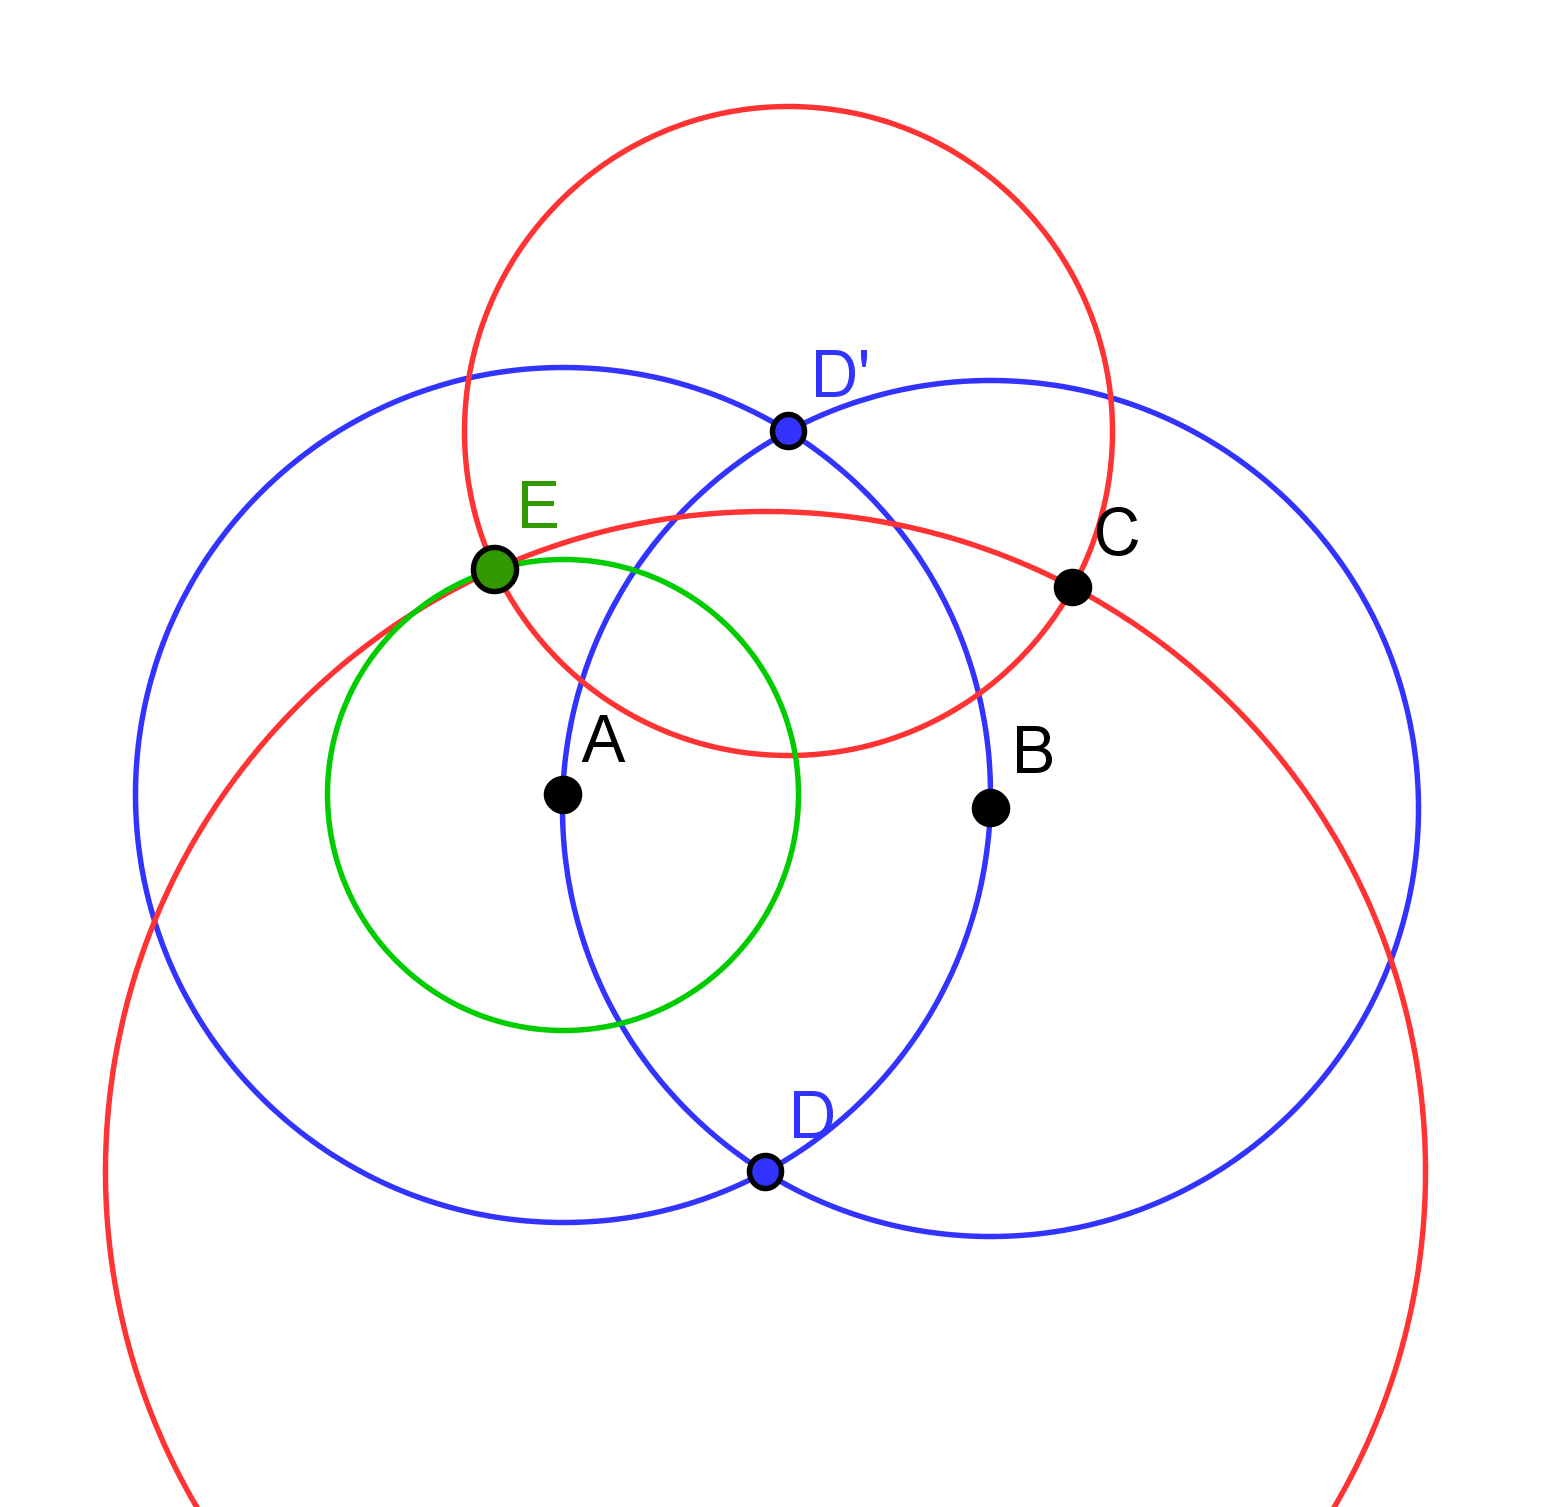
\includegraphics[width=0.65\textwidth]{CompassEquivTheorem.png}
    \caption{Færsla lengdar.}
    \label{fig:CET}
  \end{figure}
\end{frame}
\begin{frame}
  \begin{hfsmid}[Skurðpunktar hrings við línu ef línan fer ekki í gegnum
    miðju hringsins \cite{Hungerbuhler}]
    \label{hfsmid:skpomidjulinuoghrings}
    Látum hring \(\hri{MA} \Og \text{línu } \lin{P_1}{P_2}\)
    vera gefna þ.a.  \(M\) liggi ekki á línunni.
    Látum nú \(M'\) vera speglun á \(M\) um línuna \(\lin{P_1}{P_2}\).
    Við teiknum svo hring \(M'A'\) sem hring með miðju í \(M'\)
    og geisla \(MA\).
    Þá er \( X = \hri{MA} + \hri{M'A'} \) og \(Y = \hri{MA}*\hri{M'A'}\)
    skurðpunktar hringsins \(\hri{MA}\) við línuna.
    (Sjá mynd \ref{fig:mmcon1})
  \end{hfsmid}
\end{frame}

\begin{frame}
  \begin{figure}[H]
    \centering
    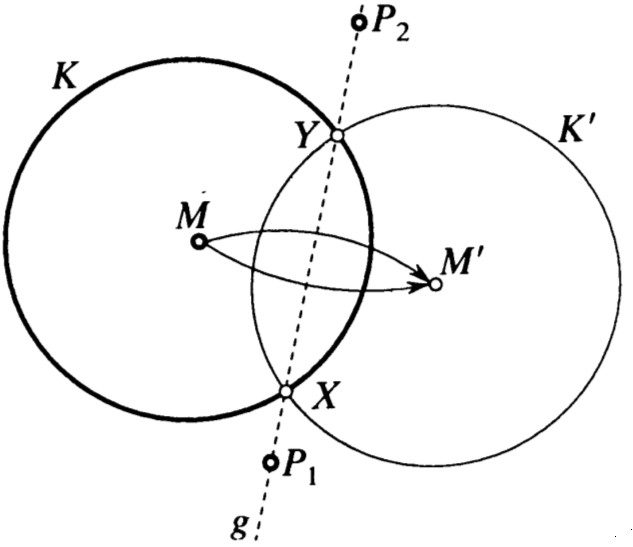
\includegraphics[width=0.5\textwidth]{MohrMaschCon1.png}
    \caption{Skurðpunktur línu og hrings (i)}
    \label{fig:mmcon1}
  \end{figure}
  En við höfum þá fundið skurðpunkt hrings og línu ef miða hringsins liggur
  ekki á línunni.
  Til þess að geta sannað (ii), þá þurfum við nokkrar smíðir í viðbót.
\end{frame}

\begin{frame}
  \begin{hfsmid}[Miðpunktur striks \cite{Hungerbuhler}] \label{hfsmid:midplinu}
    Látum \(K_1 = \hri{AB}\) og \(K_2 = \hri{BA}\).
    Finnum nú
    \(D = \hri{AB}+\hri{BA}\)
    og
    \(C = \hri{AB}*\hri{BA}\)
    Látum nú \(K_3 = \hri{CD}\)
    Finnum svo \(E = \hri{CD}*\hri{BA}\). Þá er \(B\) miðpunktur \(AE\).
    Látum nú
    \(F = \hri{EA}+\hri{AB} \) og
    \(G = \hri{EA}*\hri{AB} \).
    Þá er \(M = \hri{FA}+\hri{GA}\) miðpunktur striksins \(AB\),
    þar sem \(\Delta FAM\) og \(\Delta EFA\) eru einslægir þríhyrningar með
    hlutföll \(1:2\).
   (sjá mynd \ref{fig:mmcon2}) 
  \end{hfsmid}
\end{frame}
\begin{frame}
  \begin{figure}[H]
    \centering
    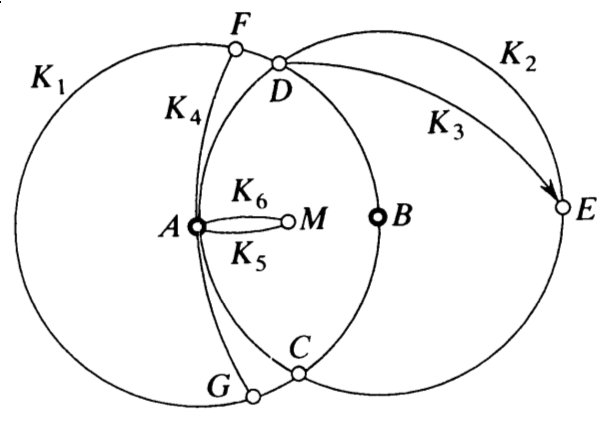
\includegraphics[width=0.5\textwidth]{MohrMaschCon2.png}
    \caption{Miðpunktur striks}
    \label{fig:mmcon2}
  \end{figure}
\end{frame}


\begin{frame}
  \begin{hfsmid}[Tvöföldun lengdar \cite{Mohr}] \label{hfsmid:tvofoldunlengdar}
    Gefum okkur tvo punkta, A og B. Látum
     \begin{gather*}
       C = \hri{AB}*\hri{BA}, D = \hri{AB}+\hri{CB}, E = \hri{AB}+\hri{DB},\\
       F = \hri{AB}+\hri{EB}, G = \hri{AB}+\hri{FB}
     \end{gather*}
     Þá mynda punktarnir \(\set{A,C,D,E,F,G}\) jafnarma sexhyrning, en sér
     í lagi er lengd striksins \(AE\) tvöföld lengd striksins
     \(AB\). (sjá mynd \ref{fig:jafnarmasexhyrningur}).

     Athugm að með því að tvöfalda lengdina \(BE\),  þá getum við fundið punkt
     \(H\) þ.a. \(AH\) sé þreföld lengd \(AB\) o.s.frv.
   \end{hfsmid}
\end{frame}
   \begin{frame}
     \begin{figure}[H]
       \centering
    \definecolor{uququq}{rgb}{0.25,0.25,0.25}
    \definecolor{qqqqff}{rgb}{0,0,1}
    \definecolor{cqcqcq}{rgb}{0.75,0.75,0.75}
    \begin{tikzpicture}[line cap=round,line join=round,>=triangle 45,x=0.8cm,y=0.8cm]
    \draw [color=cqcqcq,dash pattern=on 1pt off 1pt, xstep=0.4cm,ystep=0.4cm] (-3.12,-8.46) grid (3.69,0.2);
    \clip(-3.12,-8.46) rectangle (3.69,0.2);
    \draw(0,-4) circle (1.6cm);
    \draw(2,-4) circle (1.6cm);
    \draw(1,-2.27) circle (1.6cm);
    \draw(-1,-2.27) circle (1.6cm);
    \draw(-2,-4) circle (1.6cm);
    \draw [domain=-3.12:3.69] plot(\x,{(-0.54--1.73*\x)/1});
    \draw [domain=-3.12:3.69] plot(\x,{(-4.54-0*\x)/2});
    \draw [domain=-3.12:3.69] plot(\x,{(-0.54-1.73*\x)/1});
    \draw [domain=-3.12:3.69] plot(\x,{(--7.46-1.73*\x)/-1});
    \draw [domain=-3.12:3.69] plot(\x,{(--11.46-0*\x)/-2});
    \draw [domain=-3.12:3.69] plot(\x,{(-7.46-1.73*\x)/1});
    \draw [line width=2pt] (-2,-4)-- (-1,-5.73);
    \draw [line width=2pt] (1,-5.73)-- (2,-4);
    \draw [line width=2pt] (2,-4)-- (1,-2.27);
    \draw [line width=2pt] (-2,-4)-- (-1,-2.27);
    \draw [line width=2pt] (-1,-5.73)-- (1,-5.73);
    \draw [line width=2pt] (-1,-2.27)-- (1,-2.27);
    \draw(1,-5.73) circle (1.6cm);
    \draw(-1,-5.73) circle (1.6cm);
    \begin{scriptsize}
    \fill [color=qqqqff] (0,-4) circle (1.0pt);
    \draw[color=qqqqff] (0.07,-3.9) node {$A$};
    \fill [color=qqqqff] (2,-4) circle (1.0pt);
    \draw[color=qqqqff] (2.07,-3.9) node {$B$};
    \fill [color=uququq] (1,-2.27) circle (1.0pt);
    \draw[color=uququq] (1.08,-2.16) node {$C$};
    \fill [color=uququq] (-1,-2.27) circle (1.0pt);
    \draw[color=uququq] (-0.92,-2.16) node {$D$};
    \fill [color=uququq] (-2,-4) circle (1.0pt);
    \draw[color=uququq] (-1.92,-3.9) node {$E$};
    \fill [color=uququq] (-1,-5.73) circle (1.0pt);
    \draw[color=uququq] (-0.93,-5.63) node {$F$};
    \fill [color=uququq] (1,-5.73) circle (1.0pt);
    \draw[color=uququq] (1.08,-5.63) node {$G$};
    \end{scriptsize}
    \end{tikzpicture}
       \caption{Jafnarma sexhyrningur}
       \label{fig:jafnarmasexhyrningur}
     \end{figure}
   \end{frame}

\begin{frame}[allowframebreaks]
  \begin{hfsmid}[Skurðpunktar hrings og línu í gegnum miðju hringsins \cite{Hungerbuhler}] \label{hfsmid:skpmidjulinuoghrings}
    Látum línu \(\lin{M}{P}\) vera gefna
    Látum \(\hri{K} = \hri{MA}\) vera hring með miðju \(M\) og punkt \(A\) vera á hringnum.
    Við megum g.r.f að \(A\) sé ekki á línunni (annars finnum við  annan punkt á hringnum, t.d. með smíð \ref{hfsmid:jafnarmathri}).
    Finnum nú \(P = \hri{MA} + \lin{P}{A}\) með smíð \ref{hfsmid:skpomidjulinuoghrings} (vitum að þar sem \(A\) er ekki á línunni,
    þá er \(\lin{P}{A}\) ekki lína í gegnum miðju hringsins).
    Látum nú \(M_1\) vera miðju hrings sem fer í gegnum \(A\) og \(B\) með geisla
    sem er meiri en \(R = MA\) (getum t.d. þrefaldað lengdina \(MA\) með smíð \ref{hfsmid:tvofoldunlengdar},
    teiknað svo hring með miðju í \(A\) og \(B\) og fundið skurðpunkt þeirra.)
    Veljum svo punkt \(C = \hri{BM_1} * \hri{M_1A}\) á hringnum \(\hri{M_1A}\), og
    finnum svo \(D\) sem skurðpunkt hringsins \(\hri{M_1A}\) og hrings með miðju í
    \(C\) og geisla \(2R\).
    \theorembreak
    Finnum nú \(P' = \hri{M_1P}+\lin{C}{D}\) með smíð \ref{hfsmid:skpomidjulinuoghrings}.
    Látum nú \(M_3\) vera miðpunkt striksins \(CD\) sem við finnum með smíð \ref{hfsmid:midplinu}.
    Látum nú vera punkt á \(E = \hri{M_3C} + \hri{K_5}\) þar sem \(\hri{K_5}\) er hringur
    með miðju í \(P'\) og geisla \(PB\).
    Látum nú \(\hri{K_6}\) vera hring með miðju í \(B\) og geisla \(EC\) og
    \(\hri{K_7}\) vera hring með miðju í \(B\) og geisla \(ED\).
    Látum nú \(X \)  vera þann skurðpunkt \(\hri{K_6}\)  og \(\lin{M}{P}\)
    sem liggur á \(\hri{K}\)
    og \(Y \)  vera þann skurðpunkt \(\hri{K_7}\)  og \(\lin{M}{P}\)
    sem liggur á \(\hri{K}\)
    Þá eru \(X \Og Y \) skurðpunktar \(\lin{M}{P}\) við \(\hri{K}\).
    (sjá mynd \ref{fig:mmcon3})

  \end{hfsmid}
\end{frame}

\begin{frame}
    Þetta fæst út frá því að \(PX \cdot PY = PA \cdot PA = P'C \cdot P'D\) skv.
    reglu Eulers um sniðla sem skerast, en hún segir að
    ef tveir sniðlar hring skerast fyrir utan hringinn, þá er margfeldi hluta
    þeirra jöfn, en maður beiti því fyrst á \(\hri{MA}\) og svo á
    \(\hri{M_3C}\).

    Því eru punktarnir \(P,Y,M,X \Og B\) og
    \(P',D,M_3, C \Og E\) einslaga skv. smíð. Því eru \(X \Og Y\) fundir eins
    og sýnt var.
\end{frame}

\begin{frame}
  \begin{figure}[H]
    \centering
    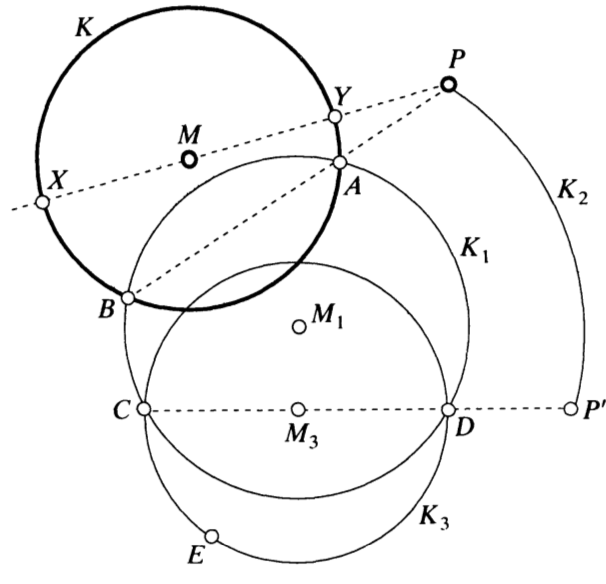
\includegraphics[width=0.5\textwidth]{MohrMaschCon3.png}
    \caption{Skurðpunktar hrings og línu í gegnum miðju hans}
    \label{fig:mmcon3}
  \end{figure}
\end{frame}

\begin{frame}
  En þar með höfum við sannað (i) og (ii) og getum því fundið skurðpunkta
  hrings og línu. Við þurfum því næst að sanna að við getum fundið skurðpunkt
  tveggja lína.
\end{frame}

\begin{frame}
  \begin{hfsmid}[Skurðpunktur línu og þverils hennar gegnum gefinn punkt \cite{Hungerbuhler}] \label{hfsmid:skplinuoghornrettarlinu}
    Látum \(\lin{P_1}{P_2}\) vera línu \(Q\) punkt. Við finnum þá punkt \(Q'\)
    með því að spegla \(Q\) um \(\lin{P_1}{P_2}\) með smíð \ref{hfsmid:speglunumlinu}.
    Við finnum svo miðpunkt striksins \(\lin{Q}{Q'}\) með smíð \ref{hfsmid:midplinu},
    en hann liggur á bæði \(\lin{Q}{Q'}\) og \(\lin{P_1}{P_2}\) og er því skurðpunktur
    þverilsins \(\lin{Q}{Q'}\) og \(\lin{P_1}{P_2}\) (sjá mynd \ref{fig:mmcon4})
  \end{hfsmid}
\end{frame}


\begin{frame}
  \begin{figure}[H]
    \centering
    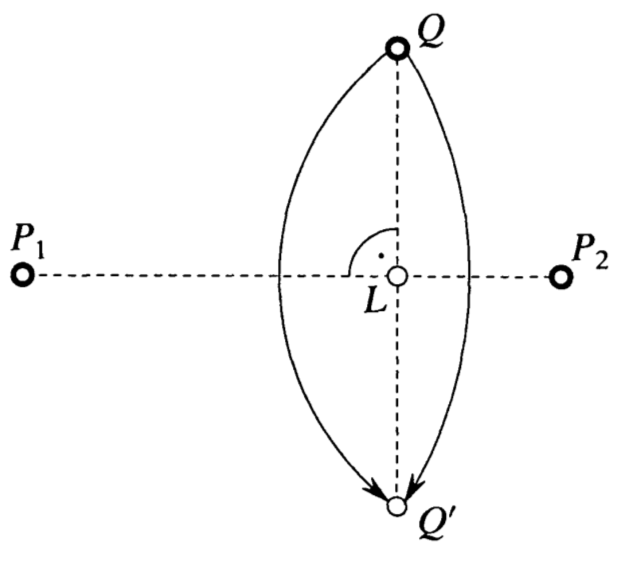
\includegraphics[width=0.6\textwidth]{MohrMaschCon4.png}
    \caption{Skurðpunktur línu og þverils hennar gegnum gefinn punkt}
    \label{fig:mmcon4}
  \end{figure}
\end{frame}

\begin{frame}
  Athugum nú hvað gerist þegar við erum með línur sem eru ekki
  hornréttar hvor á aðra (sjá mynd \ref{fig:mmcon5}).
  Það gerum við með því að finna lengdina \(l\) frá \(Q_1\) til \(S\),
  þ.e. lengdina frá einum punkti á strikinu til skurðpunktsins, en það
  gerum við í smíð \ref{hfsmid:lengdlinafraskp}.

\end{frame}

\begin{frame}
  \begin{hfsmid}[Skurðpunktur tveggja lína \cite{Hungerbuhler}]\label{hfsmid:skptveggjalina}
    Nú getum við búið til hring \(H\)
    með miðju í \(Q_1\) og geisla \(\ell\) þar sem \(\ell\)
    er fundin með smíð \ref{hfsmid:lengdlinafraskp}, en við færum
    lengdina frá punktunum \(L,E\) yfir í \(Q_1\)
    með smíð \ref{hfsmid:faerslalengdar}, en þá er \(S\)
    skurðpunktur \(H\) og \(\lin{Q_1}{Q_2}\)
    (sem við fáum úr smíð \ref{hfsmid:skpmidjulinuoghrings}).  Þá er
    \(S\) skp. \(\lin{Q_1}{Q_2} \Og \lin{P_1}{P_2}\).
  \end{hfsmid}
\end{frame}

\begin{frame}
  \begin{figure}[H]
    \centering
    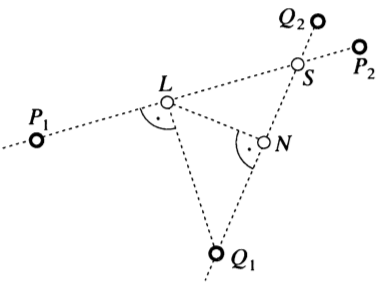
\includegraphics[width=0.5\textwidth]{MohrMaschCon5.png}
    \caption{Skurðpunktur tveggja lína}
    \label{fig:mmcon5}
  \end{figure}
\end{frame}

\begin{frame}
  Finnum nú lengdina \(\ell\):
  \begin{hfsmid}[Lengd frá punkti á striki til skurðpunkts þess við annað strik \cite{Hungerbuhler}]\label{hfsmid:lengdlinafraskp}
    Sjá mynd \ref{fig:mmcon6}.
    Við byrjum á að tvöfalda lengdina \(Q_1L\) þ.a. \(Q_1C = 2Q_1L\) með smíð
    \ref{hfsmid:tvofoldunlengdar}. Látum nú \(K\) vera hring sem er nógu stór
    (getum tvöfaldað gefnu lengdina þangað til að það dugir)
    sem fer í gegnum \(Q_1\) og \(C\) (með því að finna skurðpunkt hringja með
    geisla sem er nógu stóra lengdin og með miðjur í \(Q_1\) og \(C\)) og
    látum \(D\) vera punkt á \(\hri{K}\) þ.a. \(LD = Q_1N\) (finnum skurðpunkt
    hringsins með miðju í \(L\) og geisla \(Q_1N\)). Látum nú
    \(E\) vera skurðpunkt \(LD\) og \(\hri{K}\). Þá er lengd \(LE\) \(\ell\).
    Lengd \(LE\) er \(\ell\), þar sem \((Q_2L)^2 = Q_1L \cdot LC = LD\cdot LE = Q_1N \cdot LE\)
    skv. reglu Eulers um strengi í hring sem skerast,
    en hún segir að ef strengir í hring skerast, þá er margfeldi hluta þeirra jöfn.
    (Sjá mynd  \ref{fig:eulerschords}).
  \end{hfsmid}
\end{frame}

\begin{frame}
  \begin{figure}[H]
    \centering
    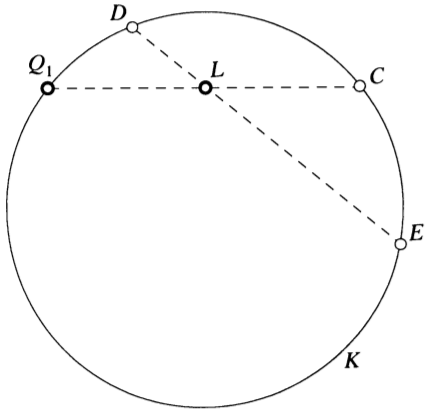
\includegraphics[width=0.5\textwidth]{MohrMaschCon6.png}
    \caption{Lengdin L fundin}
    \label{fig:mmcon6}
  \end{figure}
\end{frame}


\begin{frame}
  \begin{figure}[H]
    \centering
    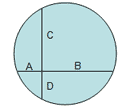
\includegraphics[width=0.2\textwidth]{EulersChords.png}
    \caption{Regla Eulers um strengi hrings sem skerast segir að \(A \cdot B = C \cdot D\) \cite{Chords}}
    \label{fig:eulerschords}
  \end{figure}
\end{frame}





  \begin{frame}
  \begin{proof}[Sönnun á Mohr-Mascheroni setningunni]
    Með því að nota smíðir \ref{hfsmid:skpmidjulinuoghrings},
    \ref{hfsmid:skpomidjulinuoghrings},
    \ref{hfsmid:skplinuoghornrettarlinu} og \ref{hfsmid:skptveggjalina},
    getum við fundið bæði skurðpunkta hrings og
    línu og skurðpunkta tveggja lína með  hringfara einum
    saman. Við vitum að við getum fundið skurðpunkta tveggja hringja
    með hringfara einum saman, og það eru einu aðgerðirnar sem
    bæta við teiknanlegum punktum. Því er sérhver mynd sem
    er teiknanleg með hringfara og reglustiku
    teiknanleg með hringfara einum saman.
  \end{proof}
\end{frame}


% \begin{frame}

%   \begin{setn}[Mohr 3.]
%     G.r.f. að við höfum gefinn hring \(\hri{AB}\). Við getum þá myndað
%     innritaðan jafnarma þríhyrning.
%   \end{setn}
%   \begin{hfsmid}
%     \(\set{B,D,F}\) í sönnuninni á (2) mynda innritaðan jafnarma þríhyrning.
%   \end{hfsmid}
% \end{frame}
% \begin{frame}
%   \begin{setn}[4. Tvöföldun lengdarinnar]
%     G.r.f að við höfum gefinn hring \(\hri{AB}\). Þá má finna punkt \(E\)
%     þ.a. \(AB = AE\) og \(E\) liggur á línunni \(A-B\).
%   \end{setn}
%   \begin{hfsmid}
%     Látum \(E\) vera eins og \(E\) í sönnuninni á (2)
%   \end{hfsmid}
% \end{frame}
% \section{Uppbygging}




\section{Poncelet-Steiner setningin}
\begin{frame}{Poncelet-Steiner setningin}
\begin{setn}[Poncelet-Steiner setningin]
Sérhverja rúmfræðilega mynd sem teikna má með hringfara og reglustiku má teikna
með reglustiku einni saman, að því gefnu að einn hringur og miðja hans sé gefin.
\end{setn}

Athugið að við þurfum að hafa gefna miðju hringsins.
Síðar var sannað að við þurfum ekki hring, heldur dugar okkur bogi með gefinni miðju.
Í teikningum með reglustiku telst hringur gefinn ef við vitum miðju hans og
geisla.
\end{frame}

\begin{frame}
  Svo virðist sem Steiner hafi gefið sér að hann mætti velja punkt af handahófi
  á þeim línum sem hann hefur nú þegar teiknað og hringnum.
  
  Athugum að ef allir punktarnir sem við fáum gefnir liggja á línunni,
  þá getum við ekki bætt við neinum punktum sem liggja ekki á línunni með
  reglustiku einni saman. Því verðum við annaðhvort að hafa að punktarnir liggi
  ekki allir á sömu línunni, eða að við megum velja okkur punkt af handahófi
  (og þá punkt sem er ekki á línunni á hringnum) á þeim hlutum sem við höfum þegar teiknað.
  Við reynum í þessari umfjöllun að sýna hvernig finna megi þessa handahófsvöldu
  punkta hjá Steiner, en það er ekki alltaf hægt. Við sleppum því því í síðari smíðum.

  \begin{figure}[H]
    \centering
    \definecolor{xdxdff}{rgb}{0.49,0.49,1}
    \definecolor{qqqqff}{rgb}{0,0,1}
    \definecolor{cqcqcq}{rgb}{0.75,0.75,0.75}
    \begin{tikzpicture}[line cap=round,line join=round,>=triangle 45,x=2.0cm,y=2.0cm]
    \draw [color=cqcqcq,dash pattern=on 1pt off 1pt, xstep=0.2cm,ystep=0.2cm] (3.25,-1.99) grid (4.38,-0.89);
    \clip(3.25,-1.99) rectangle (4.38,-0.89);
    \draw [domain=3.25:4.38] plot(\x,{(-1.12-0*\x)/0.8});
    \draw(3.94,-1.4) circle (0.53cm);
    \begin{scriptsize}
    \fill [color=qqqqff] (3.4,-1.4) circle (1.5pt);
    \draw[color=qqqqff] (3.41,-1.38) node {$A$};
    \fill [color=qqqqff] (4.2,-1.4) circle (1.5pt);
    \draw[color=qqqqff] (4.21,-1.38) node {$B$};
    \fill [color=xdxdff] (3.94,-1.4) circle (1.5pt);
    \draw[color=xdxdff] (3.95,-1.38) node {$C$};
    \end{scriptsize}
    \end{tikzpicture}
    
    \caption{Ekki er hægt að teikna þveril línunnar \(A-B\) gegnum \(A\)}
    \label{fig:ekkiallir}
  \end{figure}
\end{frame}

% \begin{frame}
%   \begin{figure}[H]
%     \centering
%     \definecolor{uququq}{rgb}{0.25,0.25,0.25}
%     \definecolor{qqqqff}{rgb}{0,0,1}
%     \begin{tikzpicture}[line cap=round,line join=round,>=triangle 45,x=0.6cm,y=0.6cm]
%     \clip(-4.06,-1.1) rectangle (6.17,5.83);
%     \draw [domain=-4.06:6.17] plot(\x,{(-0-0*\x)/4});
%     \draw(2.84,3.94) circle (0.76cm);
%     \draw [domain=-4.06:6.17] plot(\x,{(--2.54-0*\x)/0.81});
%     \draw (3.82,-1.1) -- (3.82,5.83);
%     \draw (1.86,-1.1) -- (1.86,5.83);
%     \draw [domain=-4.06:6.17] plot(\x,{(-9.26-0*\x)/-1.96});
%     \begin{scriptsize}
%     \fill [color=qqqqff] (-2,0) circle (1.5pt);
%     \draw[color=qqqqff] (-2.08,-0.28) node {$A$};
%     \fill [color=qqqqff] (0,0) circle (1.5pt);
%     \draw[color=qqqqff] (0.03,-0.28) node {$M$};
%     \fill [color=qqqqff] (2,0) circle (1.5pt);
%     \draw[color=qqqqff] (2.01,-0.28) node {$B$};
%     \fill [color=qqqqff] (2.84,3.94) circle (1.5pt);
%     \draw[color=qqqqff] (3.08,4.17) node {$O$};
%     \fill [color=uququq] (1.86,3.14) circle (1.5pt);
%     \draw[color=uququq] (1.45,2.86) node {$C$};
%     \fill [color=uququq] (3.82,4.74) circle (1.5pt);
%     \draw[color=uququq] (4.04,5.11) node {$D$};
%     \fill [color=uququq] (3.82,3.14) circle (1.5pt);
%     \draw[color=uququq] (4.04,2.94) node {$J$};
%     \fill [color=uququq] (1.86,4.74) circle (1.5pt);
%     \draw[color=uququq] (1.16,5.13) node {$K$};
%     \end{scriptsize}
%     \end{tikzpicture}
%     \caption{Smíð \ref{hogrsmid:punktfinnari}, punktfinnari (lokaútgáfa).}
%     \label{fig:punktfinnariloka}
%   \end{figure}
% \end{frame}


\begin{frame}[allowframebreaks]
  \begin{hogrsmid}[Lína samsíða gefinni stefndri línu gegnum gefin punkt P] \label{hogrsmid:samsidastefndri}
    Tveir punktar \(A \Og B\) og miðpunktur þeirra \(M\) á gefnu línunni sé þekktir.
    Köllum þetta stefnda beina línu.
    Teiknum \(A-P\) og látum \(S\) vera punkt á \(A-P\) hinumegin við \(B-P\).
    Við getum fundið \(S\) með því að nýta smíð \ref{hogrsmid:punktfinnari}
    á punkta \(A \Og P\) (eða \(B\) eða \(C\), ef við lendum í vandræðum).
    Við þurfum ekki að nota smíð \ref{hogrsmid:punktfinnari} ef við fáum
    \(S\) gefinn.
    %en ef \(M\) er í miðju gefna hringsins, þá getum við notað \(P\) \(S\)
    %sem skurðpunkt gefna hringsins við \(P-M\) (þetta er notað í smíð
    %\ref{hogrsmid:punktfinnari}).

    \theorembreak
    Teiknum svo \(S-M\) og \(B-S\). Látum \(C = B-P+ S-M\).
    Ef við teiknum svo línu \(A-C\), þá sker hún \(B-S\) í
    \(D = B-S + A-O\), en þá er línan \(P-D\) samsíða \(A-B\),
    en skv. setningu Ceva um þríhyrninga gildir \cite{WikiCeva} að þar sem
    línurnar liggja allar gegnum sameiginlegan punkt C, þá er
    
    \[\f{AM}{MB} \cdot \f{BD}{DS} \cdot \f{SP}{PA} = 1,\]
    og þar sem \(\f{AM}{BM} = 1\) er þá  \(\f{BD}{DS}= \f{PA}{SP} \)
    svo \(\f{BS}{DS}=\f{AS}{PS}\). Því eru \(\Delta ABS \equiv \Delta PDS\)
    og \(P-Q\) því samsíða \(A-B\) (því \(\angle ABS = \angle PDS\)).
  \end{hogrsmid}
\end{frame}

\begin{frame}
  \begin{figure}[H]
    \centering
    \definecolor{uququq}{rgb}{0.25,0.25,0.25}
    \definecolor{qqqqff}{rgb}{0,0,1}
    \definecolor{xdxdff}{rgb}{0.49,0.49,1}
    \definecolor{uuuuuu}{rgb}{0.27,0.27,0.27}
    \begin{tikzpicture}[line cap=round,line join=round,>=triangle 45,x=3.0cm,y=3.0cm]
    \clip(-0.22,-0.35) rectangle (2.84,1.65);
    \draw(2.49,1.11) circle (0.61cm);
    \draw [domain=-0.22:2.84] plot(\x,{(-0.36-0*\x)/-0.28});
    \draw [domain=-0.22:2.84] plot(\x,{(-0-1.14*\x)/-0.88});
    \draw [domain=-0.22:2.84] plot(\x,{(-2.27--1.14*\x)/-1.12});
    \draw [domain=-0.22:2.84] plot(\x,{(-0-0*\x)/2});
    \draw [domain=-0.22:2.84] plot(\x,{(--2.56-1.28*\x)/1.01});
    \draw (1,-0.35) -- (1,1.65);
    \draw [domain=-0.22:2.84] plot(\x,{(-0--1.02*\x)/0.99});
    \draw [domain=-0.22:2.84] plot(\x,{(--0.26-0*\x)/0.23});
    \begin{scriptsize}
    \fill [color=uuuuuu] (0,0) circle (1.0pt);
    \draw[color=uuuuuu] (0.02,0.03) node {$A$};
    \fill [color=xdxdff] (1,0) circle (1.0pt);
    \draw[color=xdxdff] (1.03,0.03) node {$M$};
    \fill [color=xdxdff] (2,0) circle (1.0pt);
    \draw[color=xdxdff] (2.02,0.03) node {$B$};
    \fill [color=qqqqff] (2.49,1.11) circle (1.0pt);
    \draw[color=qqqqff] (2.51,1.14) node {$O$};
    \fill [color=qqqqff] (0.88,1.14) circle (1.0pt);
    \draw[color=qqqqff] (0.9,1.17) node {$P$};
    \fill [color=uuuuuu] (2.60,1.29) circle (1.0pt);
    \draw[color=uuuuuu] (2.61,1.32) node {$Q$};
    \fill [color=uuuuuu] (2.40,1.29) circle (1.0pt);
    \draw[color=uuuuuu] (2.39,1.32) node {$N$}
    ;
    \fill [color=uququq] (0.99,1.28) circle (1.0pt);
    \draw[color=uququq] (1.01,1.31) node {$S$};
    \fill [color=uququq] (0.99,1.02) circle (1.0pt);
    \draw[color=uququq] (1.01,1.05) node {$C$};
    \fill [color=uququq] (1.1,1.14) circle (1.0pt);
    \draw[color=uququq] (1.12,1.17) node {$D$};
    \end{scriptsize}
    \end{tikzpicture}
    
    \caption{Lína samsíða gefinni línu gegnum gefinn punkt með punktfinnara.}
    \label{fig:samsida}
  \end{figure}
\end{frame}

\begin{frame}
  \begin{hogrsmid}[Lína samsíða gefinni línu gegnum gefinn punkt] \label{hogrsmid:samsida}
    Látum \(M-M'\) vera línuna og \(K = O|r\) vera fasta hringinn og \(P\)
    vera gefna punktinn ekki á \(M-M'\).
    Teiknum nú \(M-O\) og látum
    Notum svo smíð \ref{hogrsmid:samsidastefndri} til þess
    að finna línu samsíða \(M-O\) Í gegnum punkt á hringnum \(Y\)
    (sem við getum fundið m.þ.a. nota \(M'\) eða \(P\))
    Táknum skurðpunkt \(X-Y\) og \(M-M'\) með \(A\).
    Finnum nú \(X' \Og Y'\) sem skurðpunkta \(X-O\) við hringinn og \(Y-O\).
    Teiknum nú línu \(X' \Og Y'\) og látum \(B\) vera skurðpunkt \(X'-Y'\) við l.
    Þá er \(AM = BM\) og því eru \(A \Og B\) punktar á línunni \(M-M'\) með miðpunkt
    \(M\), en þá getum við notað smíð \ref{hogrsmid:samsidastefndri}
    til að teikna línu samsíða henni gegnum \(P\).
    Athugum að ef \(O\) er á línunni \(M-M'\), þá getum við  notað
    \(O\) og skurðpunkta \(K\) við \(M-M'\) í stað \(A, B \Og M\) og fengið
    sömu niðurstöðu.
  \end{hogrsmid}
\end{frame}

\begin{frame}
  \begin{figure}[H]
    \centering
\definecolor{uququq}{rgb}{0.25,0.25,0.25}
\definecolor{qqqqff}{rgb}{0,0,1}
\begin{tikzpicture}[line cap=round,line join=round,>=triangle 45,x=0.8cm,y=0.8cm]
\clip(-2.15,-4.91) rectangle (6.5,3.06);
\draw [domain=-2.15:6.5] plot(\x,{(-12.8--0.04*\x)/5});
\draw(1,1.54) circle (0.72cm);
\draw [domain=-2.15:6.5] plot(\x,{(-2.56--4.1*\x)/1});
\draw [domain=-2.15:6.5] plot(\x,{(-10.22--4.06*\x)/-4});
\draw [domain=-2.15:6.5] plot(\x,{(--0.65--4.1*\x)/1});
\draw [domain=-2.15:6.5] plot(\x,{(--1.03--0.28*\x)/0.85});
\draw [domain=-2.15:6.5] plot(\x,{(--1.29-0.91*\x)/-0.22});
\begin{scriptsize}
\fill [color=qqqqff] (0,-2.56) circle (1.0pt);
\draw[color=qqqqff] (0.09,-2.44) node {$M$};
\fill [color=qqqqff] (5,-2.52) circle (1.0pt);
\draw[color=qqqqff] (5.1,-2.4) node {$M'$};
\fill [color=qqqqff] (1.14,-3.7) circle (1.0pt);
\draw[color=qqqqff] (1.22,-3.59) node {$P$};
\fill [color=qqqqff] (1,1.54) circle (1.0pt);
\draw[color=qqqqff] (1.09,1.66) node {$O$};
\fill [color=uququq] (0.37,2.18) circle (1.0pt);
\draw[color=uququq] (0.45,2.29) node {$Y$};
\fill [color=uququq] (0.15,1.26) circle (1.0pt);
\draw[color=uququq] (0.22,1.38) node {$X$};
\fill [color=uququq] (1.85,1.82) circle (1.0pt);
\draw[color=uququq] (1.94,1.93) node {$X'$};
\fill [color=uququq] (1.63,0.9) circle (1.0pt);
\draw[color=uququq] (1.72,1.02) node {$Y'$};
\fill [color=uququq] (-0.78,-2.57) circle (1.0pt);
\draw[color=uququq] (-0.7,-2.45) node {$A$};
\fill [color=uququq] (0.78,-2.55) circle (1.0pt);
\draw[color=uququq] (0.87,-2.44) node {$B$};
\end{scriptsize}
\end{tikzpicture}


    \caption{Lína samsíða gefinni línu gegnum gefinn punkt}
    \label{fig:samsidalinu}
  \end{figure}
\end{frame}
\begin{frame}
  \begin{fylgismid}[Færsla gefinnar lengdar í gefinn punkt]\label{hogrsmid:faerslalengdar}
    Látum \(AB\) vera gefna lengd og \(P\) vera gefinn punkt.
    Við getum notað smíð \ref{hogrsmid:samsida} til að teikna línu \(m\) samsíða
    \(A-B\) í gegnum \(P\). Við getum einnig notað smíð \ref{hogrsmid:samsida}
    til að teikna línu \(n\) samsíða \(A-P\) í gegnum \(B\). Látum \(Q\)
    vera skurðpunkt \(l\) og \(n\). Þá er \(PQ = AM\).
    Sjá mynd \ref{fig:hogrfaerslalengdar}
  \end{fylgismid}
\end{frame}

\begin{frame}
  \begin{figure}[H]
    \centering

    \definecolor{uququq}{rgb}{0.25,0.25,0.25}
\definecolor{qqqqff}{rgb}{0,0,1}
\begin{tikzpicture}[line cap=round,line join=round,>=triangle 45,x=1.0cm,y=1.0cm]
\clip(-1.92,-4.18) rectangle (3.75,1.82);
\draw [domain=-1.92:3.75] plot(\x,{(--2.45-0*\x)/3.06});
\draw [domain=-1.92:3.75] plot(\x,{(-2.85-2.96*\x)/0.8});
\draw [domain=-1.92:3.75] plot(\x,{(-6.61-0*\x)/3.06});
\draw [domain=-1.92:3.75] plot(\x,{(--6.2-2.96*\x)/0.8});
\begin{scriptsize}
\fill [color=qqqqff] (-1.18,0.8) circle (1.0pt);
\draw[color=qqqqff] (-1.12,0.89) node {$A$};
\fill [color=qqqqff] (1.88,0.8) circle (1.0pt);
\draw[color=qqqqff] (1.95,0.89) node {$B$};
\fill [color=qqqqff] (-0.38,-2.16) circle (1.0pt);
\draw[color=qqqqff] (-0.31,-2.07) node {$P$};
\draw[color=black] (-1.84,-2.03) node {$m$};
\draw[color=black] (1.52,1.75) node {$n$};
\fill [color=uququq] (2.68,-2.16) circle (1.0pt);
\draw[color=uququq] (2.74,-2.07) node {$Q$};
\end{scriptsize}
\end{tikzpicture}
    \caption{Færsla lengdar}
    \label{fig:hogrfaerslalengdar}
  \end{figure}
  
\end{frame}

\begin{frame}
  \begin{hogrsmid}[Punktfinnari]\label{hogrsmid:punktfinnari}
    Látum \(O\) vera miðju fasta hringsins \(K\), og punkta \(P \Og A\) vera gefna. þ.a.
    \(O\) liggi ekki á \(P-A\).
    Við viljum finna punkt \(X\) þ.a. hann sé hinumegin við \(P-O\) við \(A\)
    á línunni \(A-P\).
    Teiknum \(P-O\) og látum \(C \Og D\) vera skurðpunkta \(P-O\) og \(K\).
    Teiknum svo \(A-D\) og látum \(I\) vera skurðpunkt \(A-D\) og \(K\).
    Þá getum við notað smíð \ref{hogrsmid:samsida} til
    að teikna línu samsíða \(P-O\) gegnum \(I\), þar sem að við vitum að
    punktarnir \(I\) og \(A\) eru báðir á \(A-D\) (teiknum gegnum \(A\)
    ef \(A\) er inní hringnum og endurskýrum \(A\) sem \(I\).)
    Köllum skurðpunkt línunnar við hringinn \(K\) \(L\),
    Teiknum svo línurnar \(I-O\) og köllum hinn skurðpunkt hennar við hringinn

    \(K\) \(Q\) og teiknum svo \(L-O\) og köllum hinn skurðpunkt hennar við
    hringinn \(N\). Þá er línan \(N-Q\) samsíða \(O-P\), en hinumegin við
    \(O-P\) við \(A\). Þá er skurðpunktur \(N-Q\) við \(A-P\) hinu megin við
    \(O-P\) við \(A\).
  \end{hogrsmid}
\end{frame}

\begin{frame}
  \begin{figure}[H]
    \centering
    \definecolor{uququq}{rgb}{0.25,0.25,0.25}
    \definecolor{qqqqff}{rgb}{0,0,1}
    \definecolor{xdxdff}{rgb}{0.49,0.49,1}
    \definecolor{uuuuuu}{rgb}{0.27,0.27,0.27}
    \begin{tikzpicture}[line cap=round,line join=round,>=triangle 45,x=1.0cm,y=1.0cm]
    \clip(-0.36,-1.52) rectangle (6.27,6.39);
    \draw(5.13,1.79) circle (0.83cm);
    \draw [domain=-0.36:6.27] plot(\x,{(--18.78-3*\x)/1.91});
    \draw [domain=-0.36:6.27] plot(\x,{(-0--1.79*\x)/5.13});
    \draw [domain=-0.36:6.27] plot(\x,{(-0-1.09*\x)/-5.57});
    \draw [domain=-0.36:6.27] plot(\x,{(-0-2.49*\x)/-4.68});
    \draw [domain=-0.36:6.27] plot(\x,{(--7.82-1.51*\x)/0.3});
    \draw [domain=-0.36:6.27] plot(\x,{(-4.13--0.6*\x)/-0.74});
    \draw [domain=-0.36:6.27] plot(\x,{(--6.98-1.25*\x)/0.8});
    \draw [domain=-0.36:6.27] plot(\x,{(-3.91--0.82*\x)/0.15});
    \draw [domain=-0.36:6.27] plot(\x,{(--2.49-0.21*\x)/0.8});
    \draw [domain=-0.36:6.27] plot(\x,{(--7.09-1.02*\x)/0.65});
    \draw [domain=-0.36:6.27] plot(\x,{(-0-4.78*\x)/-3.21});
    \draw [domain=-0.36:6.27] plot(\x,{(-0-0*\x)/2});
    \begin{scriptsize}
    \fill [color=uuuuuu] (0,0) circle (1.5pt);
    \draw[color=uuuuuu] (0.07,0.11) node {$A$};
    \fill [color=xdxdff] (1,0) circle (1.5pt);
    \draw[color=xdxdff] (1.08,0.11) node {$M$};
    \fill [color=xdxdff] (2,0) circle (1.5pt);
    \draw[color=xdxdff] (2.08,0.11) node {$B$};
    \fill [color=qqqqff] (5.13,1.79) circle (1.5pt);
    \draw[color=qqqqff] (5.2,1.89) node {$O$};
    \fill [color=qqqqff] (3.21,4.78) circle (1.5pt);
    \draw[color=qqqqff] (3.29,4.89) node {$P$};
    \fill [color=uuuuuu] (4.68,2.49) circle (1.5pt);
    \draw[color=uuuuuu] (4.76,2.59) node {$C$};
    \fill [color=uuuuuu] (5.57,1.09) circle (1.5pt);
    \draw[color=uuuuuu] (5.65,1.19) node {$D$};
    \fill [color=uuuuuu] (4.98,0.97) circle (1.5pt);
    \draw[color=uuuuuu] (5.03,1.07) node {$I$};
    \fill [color=uuuuuu] (4.84,1.69) circle (1.5pt);
    \draw[color=uuuuuu] (4.88,1.79) node {$J$};
    \fill [color=uuuuuu] (4.18,2.22) circle (1.5pt);
    \draw[color=uuuuuu] (4.25,2.32) node {$K$};
    \fill [color=uuuuuu] (4.32,1.99) circle (1.5pt);
    \draw[color=uuuuuu] (4.39,2.1) node {$L$};
    \fill [color=uuuuuu] (5.28,2.6) circle (1.5pt);
    \draw[color=uuuuuu] (5.35,2.71) node {$Q$};
    \fill [color=uuuuuu] (5.93,1.58) circle (1.5pt);
    \draw[color=uuuuuu] (6.01,1.69) node {$N$};
    \fill [color=uququq] (3.56,5.3) circle (1.5pt);
    \draw[color=uququq] (3.64,5.4) node {$S$};
    \end{scriptsize}
    \end{tikzpicture}
    \caption{Punktfinnari fyrir smíð \ref{hogrsmid:samsidastefndri}}
    \label{fig:punktfinnari}
  \end{figure}
\end{frame}


\begin{frame}
  \begin{hogrsmid}[Þverill línu gegnum gefinn punkt] \label{hogrsmid:thverill}
    Viljum teikna þveril línu \(l\) gegnum punkt \(P\).
    Teiknum \(l'\) með smíð \ref{hogrsmid:samsida} þ.a. hún skeri
    fasta hringinn \(K\) í \(U \Og V\). Teiknum svo strenginn
    \(U-O\) og látum \(U'\) vera skurðpunkt hans og hringsins \(K\).

    Þá er línan \(V-U'\) þverill á \(l\), en við getum svo notað
    smíð \ref{hogrsmid:samsida} til
    teikna línu samsíða \(V-U'\) í gegnum \(P\).
    Hann er þá þverill á \(l\) gegnum punkt \(P\) skv. reglu
    Þalesar \cite{WikiThales}.
  \end{hogrsmid}
\end{frame}

\begin{frame}
  \begin{figure}[H]
    \centering
    \definecolor{uququq}{rgb}{0.25,0.25,0.25}
    \definecolor{qqqqff}{rgb}{0,0,1}
    \begin{tikzpicture}[line cap=round,line join=round,>=triangle 45,x=1.0cm,y=1.0cm]
    \clip(-1.21,-3.17) rectangle (4.06,2.9);
    \draw [domain=-1.21:4.06] plot(\x,{(-6-0*\x)/3});
    \draw(1,0.5) circle (1cm);
    \draw [domain=-1.21:4.06] plot(\x,{(-3.5--2.5*\x)/-2});
    \draw [domain=-1.21:4.06] plot(\x,{(-0.83-0*\x)/3});
    \draw [domain=-1.21:4.06] plot(\x,{(-0.47--0.78*\x)/0.62});
    \draw (1.62,-3.17) -- (1.62,2.9);
    \draw (3.68,-3.17) -- (3.68,2.9);
    \begin{scriptsize}
    \fill [color=qqqqff] (0,-2) circle (1.5pt);
    \draw[color=qqqqff] (0.07,-1.92) node {$M$};
    \fill [color=qqqqff] (3,-2) circle (1.5pt);
    \draw[color=qqqqff] (3.08,-1.92) node {$M'$};
    \fill [color=qqqqff] (1,0.5) circle (1.5pt);
    \draw[color=qqqqff] (1.06,0.58) node {$O$};
    \fill [color=qqqqff] (0.89,1.49) circle (1.5pt);
    \draw[color=qqqqff] (0.96,1.58) node {$D$};
    \fill [color=qqqqff] (3.68,1.39) circle (1.5pt);
    \draw[color=qqqqff] (3.75,1.47) node {$P$};
    \fill [color=uququq] (1.62,-0.28) circle (1.5pt);
    \draw[color=uququq] (1.69,-0.19) node {$V$};
    \fill [color=uququq] (0.38,-0.28) circle (1.5pt);
    \draw[color=uququq] (0.44,-0.19) node {$U$};
    \fill [color=uququq] (1.62,1.28) circle (1.5pt);
    \draw[color=uququq] (1.7,1.36) node {$U'$};
    \end{scriptsize}
    \end{tikzpicture}
    
    \caption{Þverill gefinnar línu gegnum gefinn punkt}
    \label{fig:thverilllinu}
  \end{figure}
\end{frame}

\begin{frame}
  \begin{hogrsmid}[Strik af gefinni lengd í gefna átt frá gefnum punkti] \label{hogrsmid:strikiatt}
    Látum \(PQ\) vera gefna lengdin, \(A\) vera gefna punktinn og
    \(C-D\) vera gefna áttin.

    Byrjum á að gera línu samsíða \(C-D\) í gegnum \(A\), og köllum þá línu
    \(A-H\).
    Beitum svo fylgismíðinni og skrifum strik af lengd \(PQ\) út frá \(A\),
    og köllum hinn endapunktinn (ekki \(A\) \(K\).

    Teiknum svo línu samsíða \(C-D\) í gegnum fasta hringinn, og látum skurðpunkt hringsins
    við línuna vera \(U\). Gerum slíkt hið sama við \(P-Q\) og táknum skurðpunkt
    hringsins við hringinn með \(V\). Teiknum svo línuna \(U-V\). Teiknum
    svo línu samsíða \(U-V\) í gegnum \(K\) og finnum skurðpunkt hennar við
    \(A-H\) með \(S\). Þá er \(A-S\) samsíða \(C-D\) af lengd \(PQ\).
  \end{hogrsmid}
\end{frame}

\begin{frame}
  \begin{figure}[H]
    \centering

    \definecolor{uququq}{rgb}{0.25,0.25,0.25}
\definecolor{qqqqff}{rgb}{0,0,1}
\begin{tikzpicture}[line cap=round,line join=round,>=triangle 45,x=0.5cm,y=0.5cm]
\clip(-2.69,-5.68) rectangle (9.71,7.41);
\draw (0,-3)-- (3,-3);
\draw (-1.46,-0.12)-- (0.88,3.36);
\draw(6.32,2.38) circle (0.82cm);
\draw [domain=-2.69:9.71] plot(\x,{(-2.34--3.48*\x)/2.34});
\draw [domain=-2.69:9.71] plot(\x,{(-1.46-0.88*\x)/1.46});
\draw [domain=-2.69:9.71] plot(\x,{(--5.68-0.88*\x)/1.46});
\draw (6.32,2.38)-- (9.32,2.38);
\draw (0,-1)-- (3,-1);
\draw [domain=-2.69:9.71] plot(\x,{(-16.42--3.48*\x)/2.34});
\draw [domain=-2.69:9.71] plot(\x,{(--12.56-1.36*\x)/0.73});
\draw [domain=-2.69:9.71] plot(\x,{(--3.36-1.36*\x)/0.73});
\draw [domain=-2.69:9.71] plot(\x,{(--4.8--3.48*\x)/2.34});
\begin{scriptsize}
\fill [color=qqqqff] (0,-3) circle (1.5pt);
\draw[color=qqqqff] (0.14,-2.76) node {$P$};
\fill [color=qqqqff] (3,-3) circle (1.5pt);
\draw[color=qqqqff] (3.14,-2.76) node {$Q$};
\fill [color=qqqqff] (-1.46,-0.12) circle (1.5pt);
\draw[color=qqqqff] (-1.31,0.12) node {$C$};
\fill [color=qqqqff] (0.88,3.36) circle (1.5pt);
\draw[color=qqqqff] (1.03,3.59) node {$D$};
\fill [color=qqqqff] (6.32,2.38) circle (1.5pt);
\draw[color=qqqqff] (6.47,2.61) node {$O$};
\fill [color=qqqqff] (0,-1) circle (1.5pt);
\draw[color=qqqqff] (0.14,-0.76) node {$A$};
\fill [color=uququq] (2.34,2.48) circle (1.5pt);
\draw[color=uququq] (2.49,2.72) node {$H$};
\fill [color=qqqqff] (9.32,2.38) circle (1.5pt);
\draw[color=qqqqff] (9.51,2.61) node {$Q'$};
\fill [color=qqqqff] (3,-1) circle (1.5pt);
\draw[color=qqqqff] (3.12,-0.76) node {$K$};
\fill [color=uququq] (7.24,3.74) circle (1.5pt);
\draw[color=uququq] (7.38,3.97) node {$U$};
\fill [color=uququq] (7.96,2.38) circle (1.5pt);
\draw[color=uququq] (8.11,2.61) node {$V$};
\fill [color=uququq] (1.67,1.49) circle (1.5pt);
\draw[color=uququq] (1.81,1.72) node {$S$};
\end{scriptsize}
\end{tikzpicture}
    \caption{Færsla gefinnar lengdar í gefna átt}
    \label{fig:gefinatt}
  \end{figure}
\end{frame}

\begin{frame}
  \begin{hogrsmid}[Finnum hlutfallið milli gefinna lengda n,m og s, x = \(\f{n}{m}s\)]\label{hogrsmid:hlutfall}
    Teiknum tvo geisla út frá \(A\)
    og  notum smíð \ref{hogrsmid:strikiatt}
    til þess að merkja lengdir \(AM =m, AN = n\) á \(AB\) og \(AS = s\) á \(AC\)
    (sjá mynd \ref{fig:hlutfall}). Teiknum svo \(M-S\), og teiknum svo
    línu samsíða \(M-S\) í gegnum \(N\). Látum \(X\) tákna skurðpunkt
    hennar við \(A-C\). Þá er \(AX = x = \f{n}{m}{s}\) skv. reglu um einslaga þríhyrninga.
  \end{hogrsmid}
\end{frame}

\begin{frame}
  \begin{figure}[H]
    \centering

    \definecolor{uququq}{rgb}{0.25,0.25,0.25}
    \definecolor{xdxdff}{rgb}{0.49,0.49,1}
    \definecolor{qqqqff}{rgb}{0,0,1}
    \begin{tikzpicture}[line cap=round,line join=round,>=triangle 45,x=0.5cm,y=0.5cm]
    \clip(-1.24,-8.6) rectangle (9.79,3.53);
    \draw [domain=-1.24:9.79] plot(\x,{(-32.21--0.03*\x)/8.7});
    \draw [domain=-1.24:9.79] plot(\x,{(-31.44--5.22*\x)/8.3});
    \draw [domain=-1.24:9.79] plot(\x,{(--3.57-1.7*\x)/0.66});
    \draw [domain=-1.24:9.79] plot(\x,{(--7.26-1.7*\x)/0.66});
    \begin{scriptsize}
    \fill [color=qqqqff] (0.14,-3.7) circle (1.5pt);
    \draw[color=qqqqff] (0.25,-3.53) node {$A$};
    \fill [color=qqqqff] (8.84,-3.67) circle (1.5pt);
    \draw[color=qqqqff] (8.95,-3.5) node {$B$};
    \fill [color=qqqqff] (8.44,1.52) circle (1.5pt);
    \draw[color=qqqqff] (8.54,1.69) node {$C$};
    \fill [color=xdxdff] (2.87,-1.98) circle (1.5pt);
    \draw[color=xdxdff] (2.99,-1.81) node {$M$};
    \fill [color=xdxdff] (4.61,-0.89) circle (1.5pt);
    \draw[color=xdxdff] (4.72,-0.72) node {$N$};
    \fill [color=xdxdff] (3.53,-3.69) circle (1.5pt);
    \draw[color=xdxdff] (3.63,-3.52) node {$S$};
    \fill [color=uququq] (5.69,-3.68) circle (1.5pt);
    \draw[color=uququq] (5.79,-3.52) node {$X$};
    \end{scriptsize}
    \end{tikzpicture}
    \caption{Hlutfall milli gefinna lengda}
    \label{fig:hlutfall}
  \end{figure}
\end{frame}

\begin{frame}[allowframebreaks]
  \begin{hogrsmid}[Gefnar lengdir \(a \Og b\), smíða á \(\sqrt{ab}\)]\label{hogrsmid:kvadratrot}
    Látum \(x = \sqrt{ab}\), \(d\) vera þvermál fasta hringsins \(c\) og \(t = a+b\),
    en finna má \(t\) með því að beita smíð \ref{hogrsmid:strikiatt}.

    Látum \(h =\f{d}{t}a, \; k = \f{d}{t}b \; \Og s = \sqrt{hk}\).
    Þá er \(x = \sqrt{ab} = \sqrt{\f{th}{d} \cdot \f{tk}{d}} = \f{t}{d}s\)
    Athugum að \(h+k = d\), svo við getum búið til strik af lengd
    \(HA = h\) á miðlínu \(HK\) í hring \(c\), en þá er \(AK = k\).
    Notum smíð \ref{hogrsmid:thverill} til að búatil þverill á \(HK\) í
    gegnum \(A\) og köllum skurðpunkt þverilsins við hringinn \(S\).
    
    \theorembreak
    Þá er \(AS = \sqrt{hk}\), þar sem við höfum frá fyrirlestri Benedikts
    (og Pýþagórasi að)
    \begin{gather*}
      AS^2 + OA^2 = OS^2\\
      \Leftrightarrow AS^2 + \left(\f{d}{2} - k \right)^2 = \left(\f{d}{2} \right)^2\\
    \Leftrightarrow AS^2 = \left( \f{d}{2} \right)^2 - \left( \f{d}{2} \right)^2 + dk - k^2 \\
    \Leftrightarrow AS^2 = hk + k^2 - k^2\\
    \Leftrightarrow AS^2 = hk\\
    \Leftrightarrow AS = \sqrt{hk}
  \end{gather*}
  En þá höfum við fundið lengdirnar \(t, d \Og s\), en þá má beita
  smíð \ref{hogrsmid:hlutfall} til að finna \(x = \f{t}{d}s\)
  \end{hogrsmid}
\end{frame}

\begin{frame}
  \begin{figure}[H]
    \centering

    \definecolor{xdxdff}{rgb}{0.49,0.49,1}
    \definecolor{uququq}{rgb}{0.25,0.25,0.25}
    \definecolor{qqqqff}{rgb}{0,0,1}
    \begin{tikzpicture}[line cap=round,line join=round,>=triangle 45,x=0.6cm,y=0.6cm]
    \clip(-2.63,-8.31) rectangle (4.32,2.1);
    \draw(1,-3) circle (1.8cm);
    \draw [domain=-2.63:4.32] plot(\x,{(--9-0*\x)/-3});
    \draw (2,-8.31) -- (2,2.1);
    \draw (-0.67,-2.35) node[anchor=north west] {h};
    \draw (2.6,-2.35) node[anchor=north west] {k};
    \draw (0.5,-1.35) node[anchor=north west] {$ \sqrt{hk} $};
    \draw (1.87,-2.87)-- (2,-2.87);
    \draw (1.87,-2.87)-- (1.87,-3);
    \begin{scriptsize}
    \fill [color=qqqqff] (1,-3) circle (1.0pt);
    \draw[color=qqqqff] (1.09,-2.88) node {$O$};
    \fill [color=qqqqff] (4,-3) circle (1.0pt);
    \draw[color=qqqqff] (4.07,-2.88) node {$K$};
    \draw[color=black] (-0.48,-0.59) node {$c$};
    \fill [color=uququq] (-2,-3) circle (1.0pt);
    \draw[color=uququq] (-1.92,-2.88) node {$H$};
    \fill [color=xdxdff] (2,-3) circle (1.0pt);
    \draw[color=xdxdff] (2.09,-2.88) node {$A$};
    \fill [color=uququq] (2,-0.17) circle (1.0pt);
    \draw[color=uququq] (2.09,-0.04) node {$S$};
    \end{scriptsize}
    \end{tikzpicture}
    \caption{Finnum kvaðratrót ab}
    \label{fig:kvadratrot}
  \end{figure}
\end{frame}

\begin{frame}
  \begin{hogrsmid}[Skurðpunktar línu og hrings]\label{hogrsmid:skplinuoghrings}
    Látum \(\ell\) vera gefnu línuna og \(c = O|r\) vera gefna hringinn.
    Við þurfum að finna \(X \Og Y\), skurðpunkta \(\ell\) og \(O|r\).

    Látum \(2s\) vera lengd \(XY\), \(M\) vera miðju \(XY\) og
    \(t\) vera fjarlægðina \(OM\).

    Myndum réttan þríhyrning \(\Delta OMX\),
    en þá gefur Pýþagóras að \(s^2 = r^2 - t^2\), þ.e.
    \(s = \sqrt{(r+t)(r-t)}\).

    Þá getum við fundið \(t\) m.þ.a teikna þverill á \(\ell\) í gegnum
    \(O\) með smíð \ref{hogrsmid:thverill}. Við höfum \(r\) gefið, og
    með smíð \ref{hogrsmid:strikiatt} getum við fundið \(r+t\) og \(r-t\).
    Þá getum við beitt smíð \ref{hogrsmid:kvadratrot} til þess að finna
    \(s\), en þá getum við notað smíð \ref{hogrsmid:strikiatt} til að finna
    \(X \Og Y\).
  \end{hogrsmid}
\end{frame}

\begin{frame}
  \begin{figure}[H]
    \centering
    \definecolor{uququq}{rgb}{0.25,0.25,0.25}
    \definecolor{qqqqff}{rgb}{0,0,1}
    \begin{tikzpicture}[line cap=round,line join=round,>=triangle 45,x=1.0cm,y=1.0cm]
    \clip(0.76,-8) rectangle (4.85,-1.88);
    \draw(2.7,-4.64) circle (1.48cm);
    \draw [domain=0.76:4.85] plot(\x,{(-21.63--3.34*\x)/3.56});
    \draw [domain=0.76:4.85] plot(\x,{(--5.89--3.56*\x)/-3.34});
    \draw (2.7,-4.64)-- (1.24,-4.91);
    \begin{scriptsize}
    \draw (2.03,-4.85) node[anchor=north west] {$r$};
    \draw (2.37,-4.15) node[anchor=north west] {$t$};
    \draw (1.54,-4.25) node[anchor=north west] {$s$};
    \draw (2.30,-3.56) node[anchor=north west] {$s$};
    \end{scriptsize}
    \draw (2.21,-4.12)-- (2.15,-4.18);
    \draw (2.09,-4.11)-- (2.15,-4.18);
    \begin{scriptsize}
    \fill [color=qqqqff] (2.7,-4.64) circle (1.0pt);
    \draw[color=qqqqff] (2.75,-4.56) node {$O$};
    \draw[color=black] (1.97,-3.46) node {$c$};
    \draw[color=black] (0.8,-5.19) node {$\ell$};
    \fill [color=uququq] (1.24,-4.91) circle (1.0pt);
    \draw[color=uququq] (1.29,-4.83) node {$X$};
    \fill [color=uququq] (3.06,-3.2) circle (1.0pt);
    \draw[color=uququq] (3.11,-3.13) node {$Y$};
    \fill [color=uququq] (2.15,-4.05) circle (1.0pt);
    \draw[color=uququq] (2.21,-3.98) node {$M$};
    \end{scriptsize}
    \end{tikzpicture}
    \caption{Skurðpunktar hrings og línu}
    \label{fig:hogrskphringsoglinu}
  \end{figure}
\end{frame}

\begin{frame}[allowframebreaks]
  \begin{hogrsmid}[Skurðpunktar tveggja hringja]\label{hogrsmid:skphringja}
    Látum \(c_1 = O_1|r_1\) og \(c_2 = O_2|r_2\) vera gefnu hringina, og látum
    \(X \Og Y\) vera skurðpunkta þeirra (sem við eigum að smíða).
    Látum \(A\) vera skurðpunkt \(X-Y\) við \(O_1-O_2\).
    Látum \(t = O_1O_2, q = O_1A \Og x = XA\).
    Við þurfum að sýna að við getum smíðað lengdirnar \(q \Og x\),
    en þá getum við notað \ref{hogrsmid:strikiatt} til að finna \(A\),
    svo getum við notað \ref{hogrsmid:thverill} til að finna línuna \(X-Y\),
    og svo \ref{hogrsmid:strikiatt} aftur til að
    búa til strik af lengd \(x\) í átt \(X-Y\)til að finna \(X\) (og \(Y\)).
  \end{hogrsmid}
    %\theorembreak
  
    \begin{enumerate}[(i)]
      \item Finnum \(q\):
        Með því að nota kósínus regluna \cite{WikiCos} á
        \(\Delta O_1O_2X\) fáum við að
        \begin{align*}
          r_2^2 & = r_1^2 + t^2 - 2r_1 t \cos{(\angle XO_1O_2)}\\
                & = r_1^2 + t^2 - 2t(r_1  \cos{(\angle XO_1O_2)}) \;\;\;(*)\\
                & = r_1^2 + t^2 - 2tq
        \end{align*}
        (\((*)\)
        sjá mynd \ref{fig:acuteangle} frá Wikipediu \cite{WikiCos}).
        Látum \(d = \sqrt{r_1^2 + t^2}\),
        en þá er \(q = \f{(d+r_2)(d-r_2)}{2t}\).
        \(d\)
        er langhlið rétthyrnds þríhyrnings með skammhliðar \(r_1\)
        og \(r_2\)
        er hægt að búa til með \ref{hogrsmid:thverill} og
        \ref{hogrsmid:strikiatt}, og ef við látum svo \(n = d+r_2\),
        \(m = 2t\)
        og \(s = d_2 -r_2\),
        þá eru þær lengdir allar smíðanlegar með
        \ref{hogrsmid:strikiatt} og \(q = \f{n}{m}s\)
        er smíðanleg með \ref{hogrsmid:hlutfall}.
      \item Finnum \(x\):
        Athugum að \(\Delta AO_1X\)
        mynda rétthyrndan þríhyrning, svo \(x^2 = r^2 - q^2\),
        svo \(x = \sqrt{r_1+q}{r_1-q}\).
        Með smíð \ref{hogrsmid:strikiatt} getum við búið til
        \(h = r_1 +q\)
        og \(k = r_1 - q\),
        en þá getum við notað smíð \ref{hogrsmid:kvadratrot} til að
        finna \(\sqrt{hk}\).

    \end{enumerate}
    En með (i) og (ii) höfum við þá fundið \(q \Og x\) og getum þar með
    fundið \(X \Og Y\).
\end{frame}


\begin{frame}
  \begin{figure}[H]
    \centering
    \definecolor{uququq}{rgb}{0.25,0.25,0.25}
    \definecolor{qqqqff}{rgb}{0,0,1}
    \begin{tikzpicture}[line cap=round,line join=round,>=triangle 45,x=1.3cm,y=1.3cm]
    \clip(-0.94,-2.97) rectangle (2.5,2.18);
    \draw(-0.56,-0.42) circle (2.6cm);
    \draw(1.91,-0.41) circle (1.3cm);
    \draw [domain=-0.94:2.5] plot(\x,{(-1.03--0.01*\x)/2.47});
    \draw (-0.56,-0.42)-- (1.28,0.37);
    \draw (1.28,0.37)-- (1.91,-0.41);
    \draw (1.28,0.37)-- (1.28,-1.2);
    \begin{scriptsize}
    \draw (0.56,-0.40) node[anchor=north west] {$q$};
    \draw (1.10,-0.05) node[anchor=north west] {$x$};
    \fill [color=qqqqff] (-0.56,-0.42) circle (1.0pt);
    \draw[color=qqqqff] (-0.48,-0.36) node {$O_1$};
    \draw[color=black] (-1.5,1.21) node {$c_1$};
    \fill [color=qqqqff] (1.91,-0.41) circle (1.0pt);
    \draw[color=qqqqff] (1.99,-0.35) node {$O_2$};
    \draw[color=black] (1.46,0.37) node {$c_2$};
    \fill [color=uququq] (1.28,0.37) circle (1.0pt);
    \draw[color=uququq] (1.32,0.43) node {$X$};
    \fill [color=uququq] (1.28,-1.2) circle (1.0pt);
    \draw[color=uququq] (1.32,-1.13) node {$Y$};
    \draw[color=black] (0.44,-0.06) node {$r_1$};
    \draw[color=black] (1.57,-0.04) node {$r_2$};
    \fill [color=uququq] (1.28,-0.42) circle (1.0pt);
    \draw[color=uququq] (1.32,-0.36) node {$A$};
    \end{scriptsize}
    \end{tikzpicture}
    \caption{Skurðpunktar tveggja hringja}
    \label{fig:hogrskptveggjahringja}
  \end{figure}
\end{frame}

\begin{frame}
  \begin{figure}[H]
    \centering
    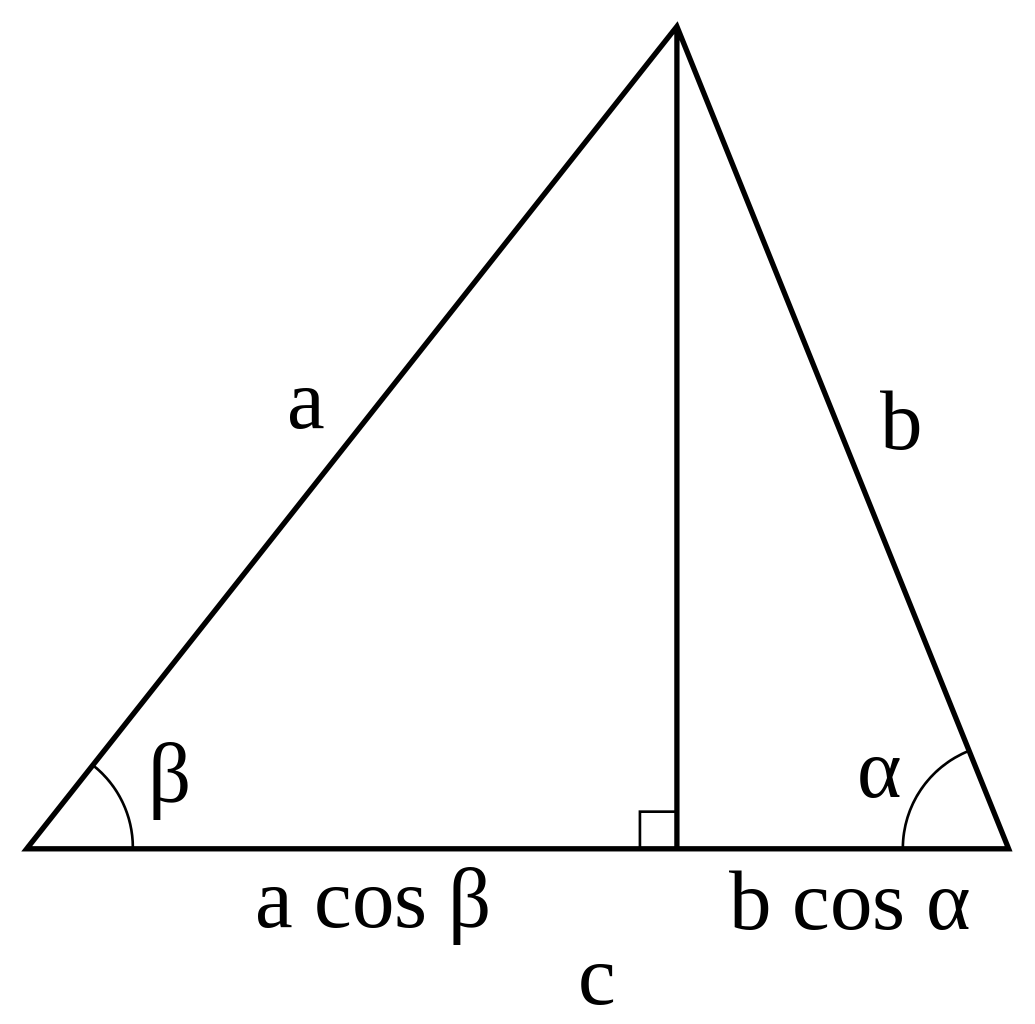
\includegraphics[width=0.6\textwidth]{AcuteAngle.png}
    \caption{Útskýring á að \(r_1 \cos{(\angle XO_1O_2)} = q \)}
    \label{fig:acuteangle}
  \end{figure}
\end{frame}

\begin{frame}{Poncelet-Steiner setningin}
  \begin{proof}[Sönnun á Poncelet-Steiner setningunni]
    Með því að nota smíðir \ref{hogrsmid:skplinuoghrings} og \ref{hogrsmid:skphringja}
    getum við fundið skurðpunkta hrings og línu og skurðpunkta
    tveggja hringja með einum hring og reglustiku. Þar sem við getum þegar
    fundið skurðpunkt tveggja lína með reglustiku, þá getum við  beitt öllum
    aðgerðunum sem bæta við teiknanlegum punktum. Því er sérhver mynd sem er
    teiknanleg með hringfara og reglustiku teiknanleg með reglustiku og einum
    hring.
\end{proof}
\end{frame}

\section{Þrískipting horns og annað ómögulegt} 

\begin{frame}
  Dæmi eru til um sléttumyndir sem ekki er hægt að mynda með einungis hringfara og reglustiku
\begin{itemize}
\item Þrískipting horns. Verkefnið felst í að mynda línur sem skipta gefnu horni í þrjú jafn stór horn. Sannað af Pierre Wantzel árið 1837 (með hjálp Galois fræði).
\item Ferningun hrings. Verkefni felst í að búa til ferning sem hefur sama flatarmál og 
gefinn hringur. Ekki hægt, þar sem það krefst torræðar tölu (\(\sqrt{\pi}\)). (sjá sönnun hjá Jóni Áskeli síðar í samæfingum.)
\item Tvöföldun tenings. Verkefnið felst í að búa til hlið fernings sem hefur tvöfalt rúmmál á við gefin tening. Ekki hægt, því ekki er hægt að mynda \(\sqrt{3}{2}\) úr heilutölunum með
samlagningu, frádrætti, margföldun, deilingu og kvaðratrótum.
\end{itemize}
\end{frame}

\begin{frame}
  Þó er hægt að þrískipta horni, ef við leyfum okkur reglustiku sem er merkt
  á tveimur stöðum. Til þess þurfum við þó fleiri smíðir.
\end{frame}

\begin{frame}
  \begin{smid}[Tvískipting horns \cite{Bisect}]
    \label{smid:tviskiptinghorns}
    Látum horn \(\angle PQR\) vera gefið.
    Finnum miðpunkt \(PQ\) með smíð \ref{hfsmid:midplinu}
    og köllum \(M\).
    Teiknum hringinn \(\hri{QM}\) og finnum skurðpunktinn
    \(P_1 = \lin{Q}{P}+\hri{QM}\)  og skurðpunktinn \(P_2 = \lin{Q}{R}+\hri{QM}\)
    Finnum einnig  skurðpunktinn
    \(S_1 = \lin{Q}{P}+\hri{QP}\)  og skurðpunktinn \(S_2 = \lin{Q}{R}+\hri{QP}\)
    Þá er lengd striksins \(S_1P_1\) sú sama og lengd striksins
    \(S_2P_2\).
    Teiknum nú skurðpunkt hringjana
    \(C = \hri{S_1P_1}+\hri{S_2P_2}\).
    Þá helmingar línan \(\lin{Q}{C}\) hornið \(\angle PQR\).
  \end{smid}
\end{frame}

\begin{frame}
  Við sjáum að með því að beita smíð \ref{smid:tviskiptinghorns}, þá getum við
  breytt hvaða horni í summu hvassra horna. Við getum svo þrískipt hverju horni fyrir
  sig, og notað svo þær þrískiptingar til að mynda þrískiptingu upprunalega hornsins.
\end{frame}

\begin{frame}[allowframebreaks]
  \begin{smid}[Þrískipting horns með tvímerktri reglustiku \cite{Baragar}]
    \label{smid:thriskipting}
    Látum hvasst horn \(\alpha\)
    með oddpunkt \(O\)
    vera gefið. Látum nú annað merki reglustikunnar í \(O\)
    og merkjum punkt \(D\)
    við hina merkinguna. Strikið \(\lin{O}{D}\)
    hefur þá lengdina \(d\).
    Teiknum nú hring \(\hri{OD}\).
    Finnum nú nú skp. arma hornsins við hringinn \(\hri{OD}\)
    og köllum þá
    \(A \Og B\). Þá er \(\alpha = \angle\, AOB\). Teiknum nú línuna \(OA\).

    \theorembreak
    
    Látum nú reglustikuna þannig að önnur merkingin er á hringnum hinumegin
    við línuna \(\lin{O}{B}\) við \(A\), og hin sömu megin á línunni \(\lin{O}{A}\),
    og reglustikan fer í gegnum punkt \(B\). Köllum þá \(R \Og Q\). Látum nú
    \(\beta = \angle\, RQO\). Þá er þríhyrningurinn \(\Delta\, RQO\) jafnarma,
    þar sem \(|RQ| = |RO|\). Því er \(\angle\, ROQ = \beta\) og því er
    \(\angle\, BRO = 2 \beta\). Þar sem þríhyrningurinn \(\Delta\, BRO\)
    er líka jafnarma, \(\angle\, RBO = \angle\, BRO = 2\beta\). En þá er
    \(\angle\, ROB = \pi - 4\beta\) (hornasumma þríhyrnings í radíönum er \(\pi\)).
    Með því að summera upp hornin í \(O\) fæst því að
    \[ \beta + (\pi - 4\beta) + \alpha = \pi,\]
    en það þýðir að \(\alpha = 3\beta\)
  \end{smid}
\end{frame}

\begin{frame}
  \begin{figure}[H]
    \centering
    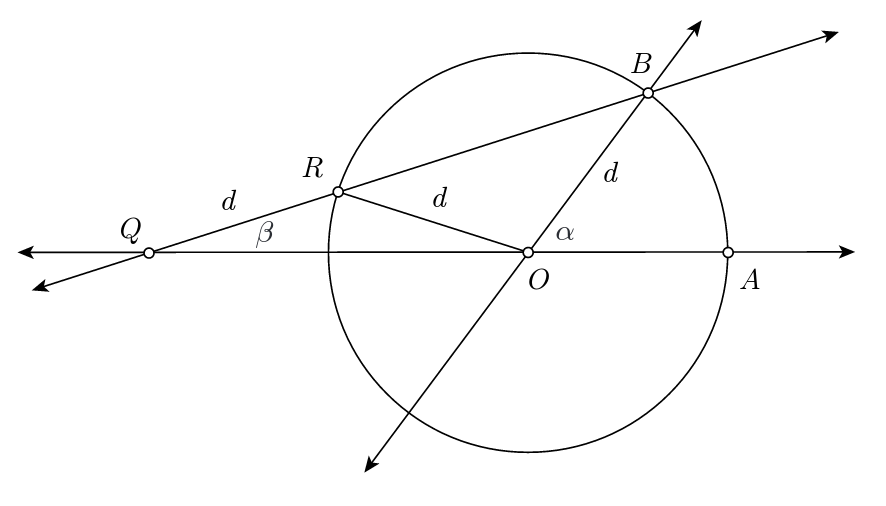
\includegraphics[width=0.8\textwidth]{TwiceNotched.png}
    \caption{Þrískipting horns með tvímerktri reglustiku}
    \label{fig:thriskipt}
  \end{figure}
\end{frame}

\begin{frame}
  Vert er að nefna að með því að nota japönsk pappírsbrotslistina
  Origami \cite{WikiOrigami}, þá má tvöfalda
  teninginn og þrískipta horninu. Þar eru aðgerðirnar gefnar með
  Huzita-Hatori forsendunum \cite{WikiHuzita}.
  \begin{figure}[H]
    \centering
    \begin{subfigure}[]{0.4\textwidth}
      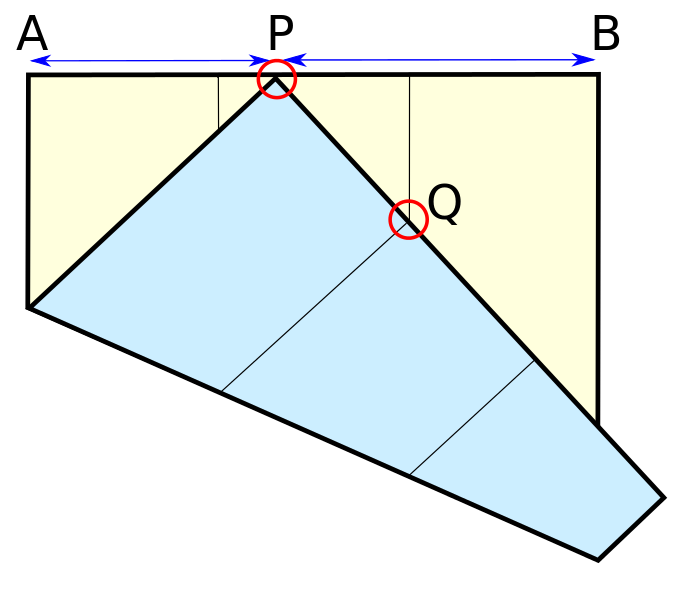
\includegraphics[width=\textwidth]{CubeDoublingOrigami}
      \subcaption{\(PB/PA = \sqrt[3]{2}\)}
    \end{subfigure}
    \begin{subfigure}[]{0.4\textwidth}
      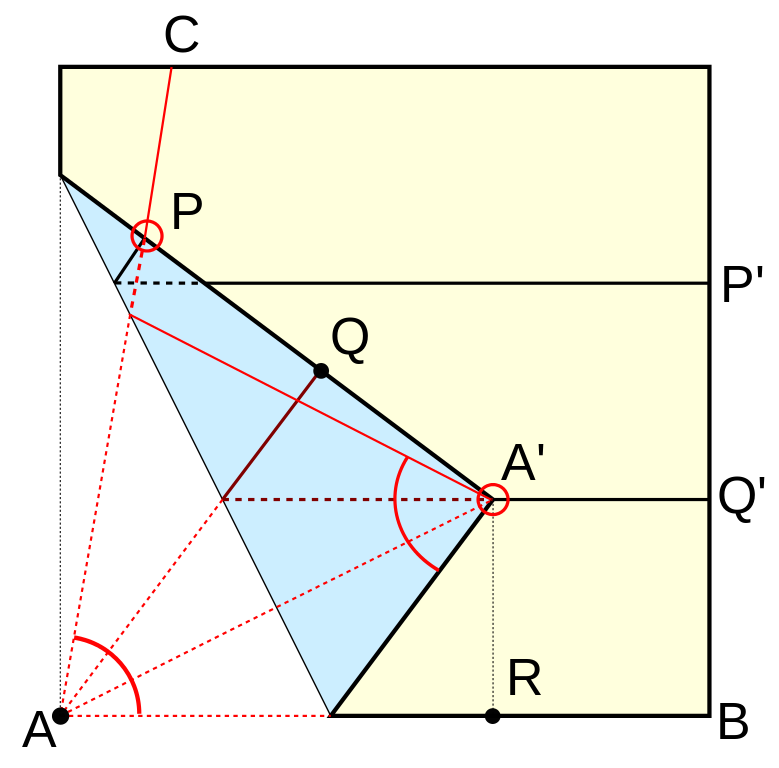
\includegraphics[width=\textwidth]{AngleTrisectionOrigami}
      \subcaption{Þrískipting hornsins \(CAB\)}
    \end{subfigure}
    \caption{Tvöföldun tengingsins og þrískipting hornsins með Origami}
    \label{fig:origami}
  \end{figure}
  
\end{frame}


\section{Heimildir}
\begin{frame}[allowframebreaks]

  \frametitle<presentation>{Heimildir} 
  
  \begin{thebibliography}{10}    
  \beamertemplateonlinebibitems
  \bibitem{WikiCasc}
     Wikipedia
     \newblock {\em Compass-and-straightedge construction}.
     \newblock \url{http://en.wikipedia.org/w/index.php?title=Compass-and-straightedge_construction&oldid=642473603}
     \newblock Online; accessed 18-January-2015.
  \bibitem{WikiCET}
     Wikipedia
     \newblock {\em Compass-equivalence theorem}.
     \newblock \url{https://en.wikipedia.org/w/index.php?title=Compass_equivalence_theorem&oldid=637959570}
     \newblock Online; accessed 29-January-2015.
  \bibitem{WikiMMt}
     Wikipedia
     \newblock {\em Mohr-Mascheroni theorem}.
     \newblock \url{http://en.wikipedia.org/w/index.php?title=Mohr%E2%80%93Mascheroni_theorem&oldid=614723343
     }
     \newblock Online; accessed 20-January-2015.

   \bibitem{WikiCeva}
     Wikipedia
     \newblock {\em Ceva's theorem}.
     \newblock \url{https://en.wikipedia.org/w/index.php?title=Ceva%27s_theorem&oldid=633406630
     }
     \newblock Online; accessed 30-January-2015.
   \bibitem{WikiThales}
     Wikipedia
     \newblock {\em Thales's theorem}.
     \newblock \url{https://en.wikipedia.org/w/index.php?title=Thales%27_theorem&oldid=643678036
     }
     \newblock Online; accessed 30-January-2015.
   \bibitem{WikiCos}
     Wikipedia
     \newblock {\em Law of cosines}.
     \newblock \url{https://en.wikipedia.org/w/index.php?title=Law_of_cosines&oldid=645015128}
     \newblock Online; accessed 1-Febuary-2015.
     
  \bibitem{WikiPSt}
     Wikipedia
     \newblock {\em Poncelet-Steiner theorem}.
     \newblock  \url{http://en.wikipedia.org/w/index.php?title=Poncelet%E2%80%93Steiner_theorem&oldid=614055164
     }.
     \newblock Online; accessed 20-January-2015.
  \bibitem{WikiOrigami}
     Wikipedia
     \newblock {\em Mathematics of paper folding}.
     \newblock  \url{https://en.wikipedia.org/w/index.php?title=Mathematics_of_paper_folding&oldid=630113885}.
     \newblock Online; accessed 1-Febuary-2015.
     
  \bibitem{WikiHuzita}
     Wikipedia
     \newblock {\em Huzita–Hatori axioms}.
     \newblock  \url{https://en.wikipedia.org/w/index.php?title=Huzita%E2%80%93Hatori_axioms&oldid=591740270
     }.
     \newblock Online; accessed 1-Febuary-2015.
   \bibitem{Chords}
     Math Open Reference.
     \newblock {\em Intersecting Chord Theorem}.
     \newblock \url{http://www.mathopenref.com/chordsintersecting.html}.
     \newblock Online; accessed 28-January-2015.

   \bibitem{Chords}
     Math Open Reference.
     \newblock {\em Intersecting Secants Theorem}.
     \newblock \url{http://www.mathopenref.com/secantsintersecting.html}.
     \newblock Online; accessed 29-January-2015.
   \bibitem{Bisect}
     Math Open Reference.
     \newblock {\em  Bisecting an Angle}.
     \newblock \url{http://www.mathopenref.com/constbisectangle.html}.
     \newblock Online; accessed 28-January-2015.
     
  \beamertemplatearticlebibitems
  \bibitem{Baragar}
     Arthur Baragar.
     \newblock {\em Constructions Using a Compass and Twice-Notched Straightedge}.
      \newblock The American Mathematical Monthly, Vol. 109, No. 2 (Feb., 2002), pp. 151-164.
      \newblock  \url{http://www.jstor.org/stable/2695327}.
    \bibitem{Woltermann}
      Michael Woltermann.
      \newblock {\em Steiner’s Straight-edge Problem}.
      \newblock  \url{http://www2.washjeff.edu/users/mwoltermann/Dorrie/34.pdf}.
      
    \bibitem{Hungerbuhler}
      Norbert Hungerbuhler.
      \newblock {\em A Short Elementary Proof of the Mohr-Mascheroni Theorem}.
      \newblock The American Mathematical Monthly, Vol. 101, No. 8 (Oct., 1994), pp. 784-787.
      %Published by: Mathematical Association of America
      \newblock \url{http://www.jstor.org/stable/2974536}.
  \beamertemplatebookbibitems
\bibitem{Mohr}
  Jørgen Mohr.
  \newblock {\em Euclidus Danicus}.
  \newblock Amsterdam: Van Velsen, 1672 (København: 1928).
  
\bibitem{Euclid}
  Evklíð.
  \newblock John Casey.
  \newblock {\em The First Six Books of the Elements of Euclid }
  \newblock \url{www.gutenberg.org/ebooks/21076}
\bibitem{Reynir}
  Reynir Axelsson.
  \newblock {\em Kafli um teiknanlega punkta úr bók um evklíðska rúmfræði}.
  \newblock Óútgefið.
  \end{thebibliography}
\end{frame}

\end{document}
